    %%%%%%%%%%%%%%%%%%%%%%%%%%%%%%%%%%%%%%%%%%%%%%%%%%%%%%%%%%%%%%%%%%%%%%%%%%%%%%%
%Objetivo: Descrever os principais conceitos relativos a Manutenção de Software
%		   envolvidos na dissertação
%Autores: Vagner Clementino <vagnercs@dcc.ufmg.br>
%		  Rodolfo Resende <rodolfo@dcc.ufmg.br>
%Criação: Ter Set 13 19:22:37 BRT 2016
%Modificação: qua set 13 22:49:56 -03 2017
%Revisão: sáb mai 27 17:13:26 -03 2017
%%%%%%%%%%%%%%%%%%%%%%%%%%%%%%%%%%%%%%%%%%%%%%%%%%%%%%%%%%%%%%%%%%%%%%%%%%%%%%%

\chapter{As FGRMs no Contexto da Manutenção de Software}\label{ch:visao-geral-manutencao}

Os sistemas de software têm tendência de evoluir para atender  aos requisitos e
alterações do ambiente no qual eles se inserem. Em uma série de estudos, Lehman
propôs leis sobre a evolução do software. A Lei da Mudança Contínua
(\textit{Continuing Change}) afirma que um software em uso deve mudar ou se
tornará progressivamente menos útil~\cite{lehman1980understanding}. A Lei da
Complexidade Crescente (\textit{Increasing complexity}) afirma que as mudanças
realizadas em um sistema transforma sua estrutura cada vez mais complexa. Neste
contexto, recursos extras devem ser disponibilizados a fim de preservar e
simplificar a estrutura do software~\cite{lehman1980understanding}. As leis de
Lehman têm sido validadas, especialmente aquelas relacionadas ao tamanho e
complexidade do software. Em um trabalho sobre o tema Yu e
Mishra~\cite{{yu2013empirical}} examinaram de forma empírica as Leis de Lehman
em relação à evolução da qualidade do software. O estudo demonstrou que a
qualidade declinará a menos que sejam realizadas modificações com objetivo de
melhoria da qualidade do produto.

Partindo da premissa de que mudanças em software são inevitáveis, torna-se
importante uma disciplina com foco no gerenciamento e controle das alterações.
Em geral, dentro do escopo da Engenharia de Software a tarefa fica a cargo da
\textit{Manutenção de Software}. Nas próximas seções discutimos os conceitos
básicos da Manutenção de Software que foram utilizados nesta dissertação e sua
relação com as FGRMs.

\section{A Manutenção de Software e a Requisição de Mudança}\label{sec:conceitos_basicos}

Nesta seção apresentamos os vários termos e conceitos relacionados à Manutenção
de Software e a relação destes termos com o conceito de Requisição de Mudança.
Iniciamos com uma visão geral da Manutenção de Software.

\subsection{Visão Geral da Manutenção de Software}\label{sub:visão_geral_da_manutenção_de_softare}

No Padrão IEEE 1219~\cite{ISO-1219-1998} a Manutenção de Software é definida
como a modificação de um produto de software após a sua entrega com o objetivo
de corrigir falhas, melhorar o desempenho ou outros atributos com a finalidade
de adaptar o sistema às modificações ambientais.

Posteriormente a IEEE/EIA 12207~-~Padrão para o Processo de Ciclo de Vida do
Software~\cite{ISOIEC-12207-2008}, retrata a manutenção como um dos principais
processos no ciclo de vida do software. Em seu texto a disciplina corresponde
às atividades de modificação do código e da documentação associada em
decorrência de uma falha ou necessidade de melhoria no
software~\cite{IEEEComputerSociety:2014:GSE:2616205}.

De maneira relacionada, \textit{Manutenibilidade} é a propriedade de um sistema
ou componente de software em relação ao grau de \textit{facilidade} que ele pode
ser corrigido, melhorado ou adaptado~\cite{{159342}}. A
ISO/IEC~9126~-~01~\cite{ISOIEC9126} define a Manutenibilidade como um atributo
de qualidade do processo de Manutenção.

É possível verificar que  \textit{manter e evoluir} são aspectos comuns das
diferentes definições para Manutenção de Software. Embora exista o entendimento
que os processos de manutenção e evolução possuem características
distintas~\cite{tripathy2014software}, não está nos objetivos desta dissertação
discutir e apresentar as diferenças. Neste sentido, utilizamos ambos os termos
de forma intercambiáveis.

\subsection{O Processo de Manutenção de Software}\label{sec:o_processo_de_manutecao_de_software}

O Processo de Manutenção de Software é caracterizado pelo conjunto de
atividades, métodos, práticas e transformações utilizadas para desenvolver ou
manter um software e seus artefatos associados~\cite{paulk1993key}. Existe na
literatura alguns modelos para o processo de manutenção de software,
especialmente baseados em uma visão ``tradicional''. Nesta perspectiva o
desenvolvimento e a manutenção de software possuem uma separação clara.
Contudo, no momento do desenvolvimento desta dissertação, existia uma tendência
cada vez maior da adoção das práticas propostas pelos agilistas na manutenção
de software. Esta inclinação surge da demanda por serviços de manutenção de
rápido retorno para o usuário.

\subsubsection{Manutenção de Software Tradicional}\label{subsec:manutenção_de_software_tradicional}

Nesta seção apresentamos e discutimos alguns modelos para o processo de
manutenção, que segundo o nosso entendimento, são os principais disponíveis na
literatura. No contexto desta dissertação estes modelos são descritos como
tradicionais. Em resumo, um processo de manutenção de software descreve as
atividades e suas respectivas entradas e saídas. Alguns modelos são descritos
nos padrões IEEE~1219~\cite{IEEE1999-Std1219} e
ISO/IEC~14764~\cite{institute2006norma}. O processo especificado no padrão IEEE
1219 prescreve que as atividades de manutenção de software devem ser iniciadas
após a entrega do produto de software. O padrão também discute aspectos de
planejamento da manutenção. As atividades que compõem o processo são
apresentadas na Figura~\ref{fig:ieee-1219-processo-man-software}.

\begin{figure}[htpb] \centering
    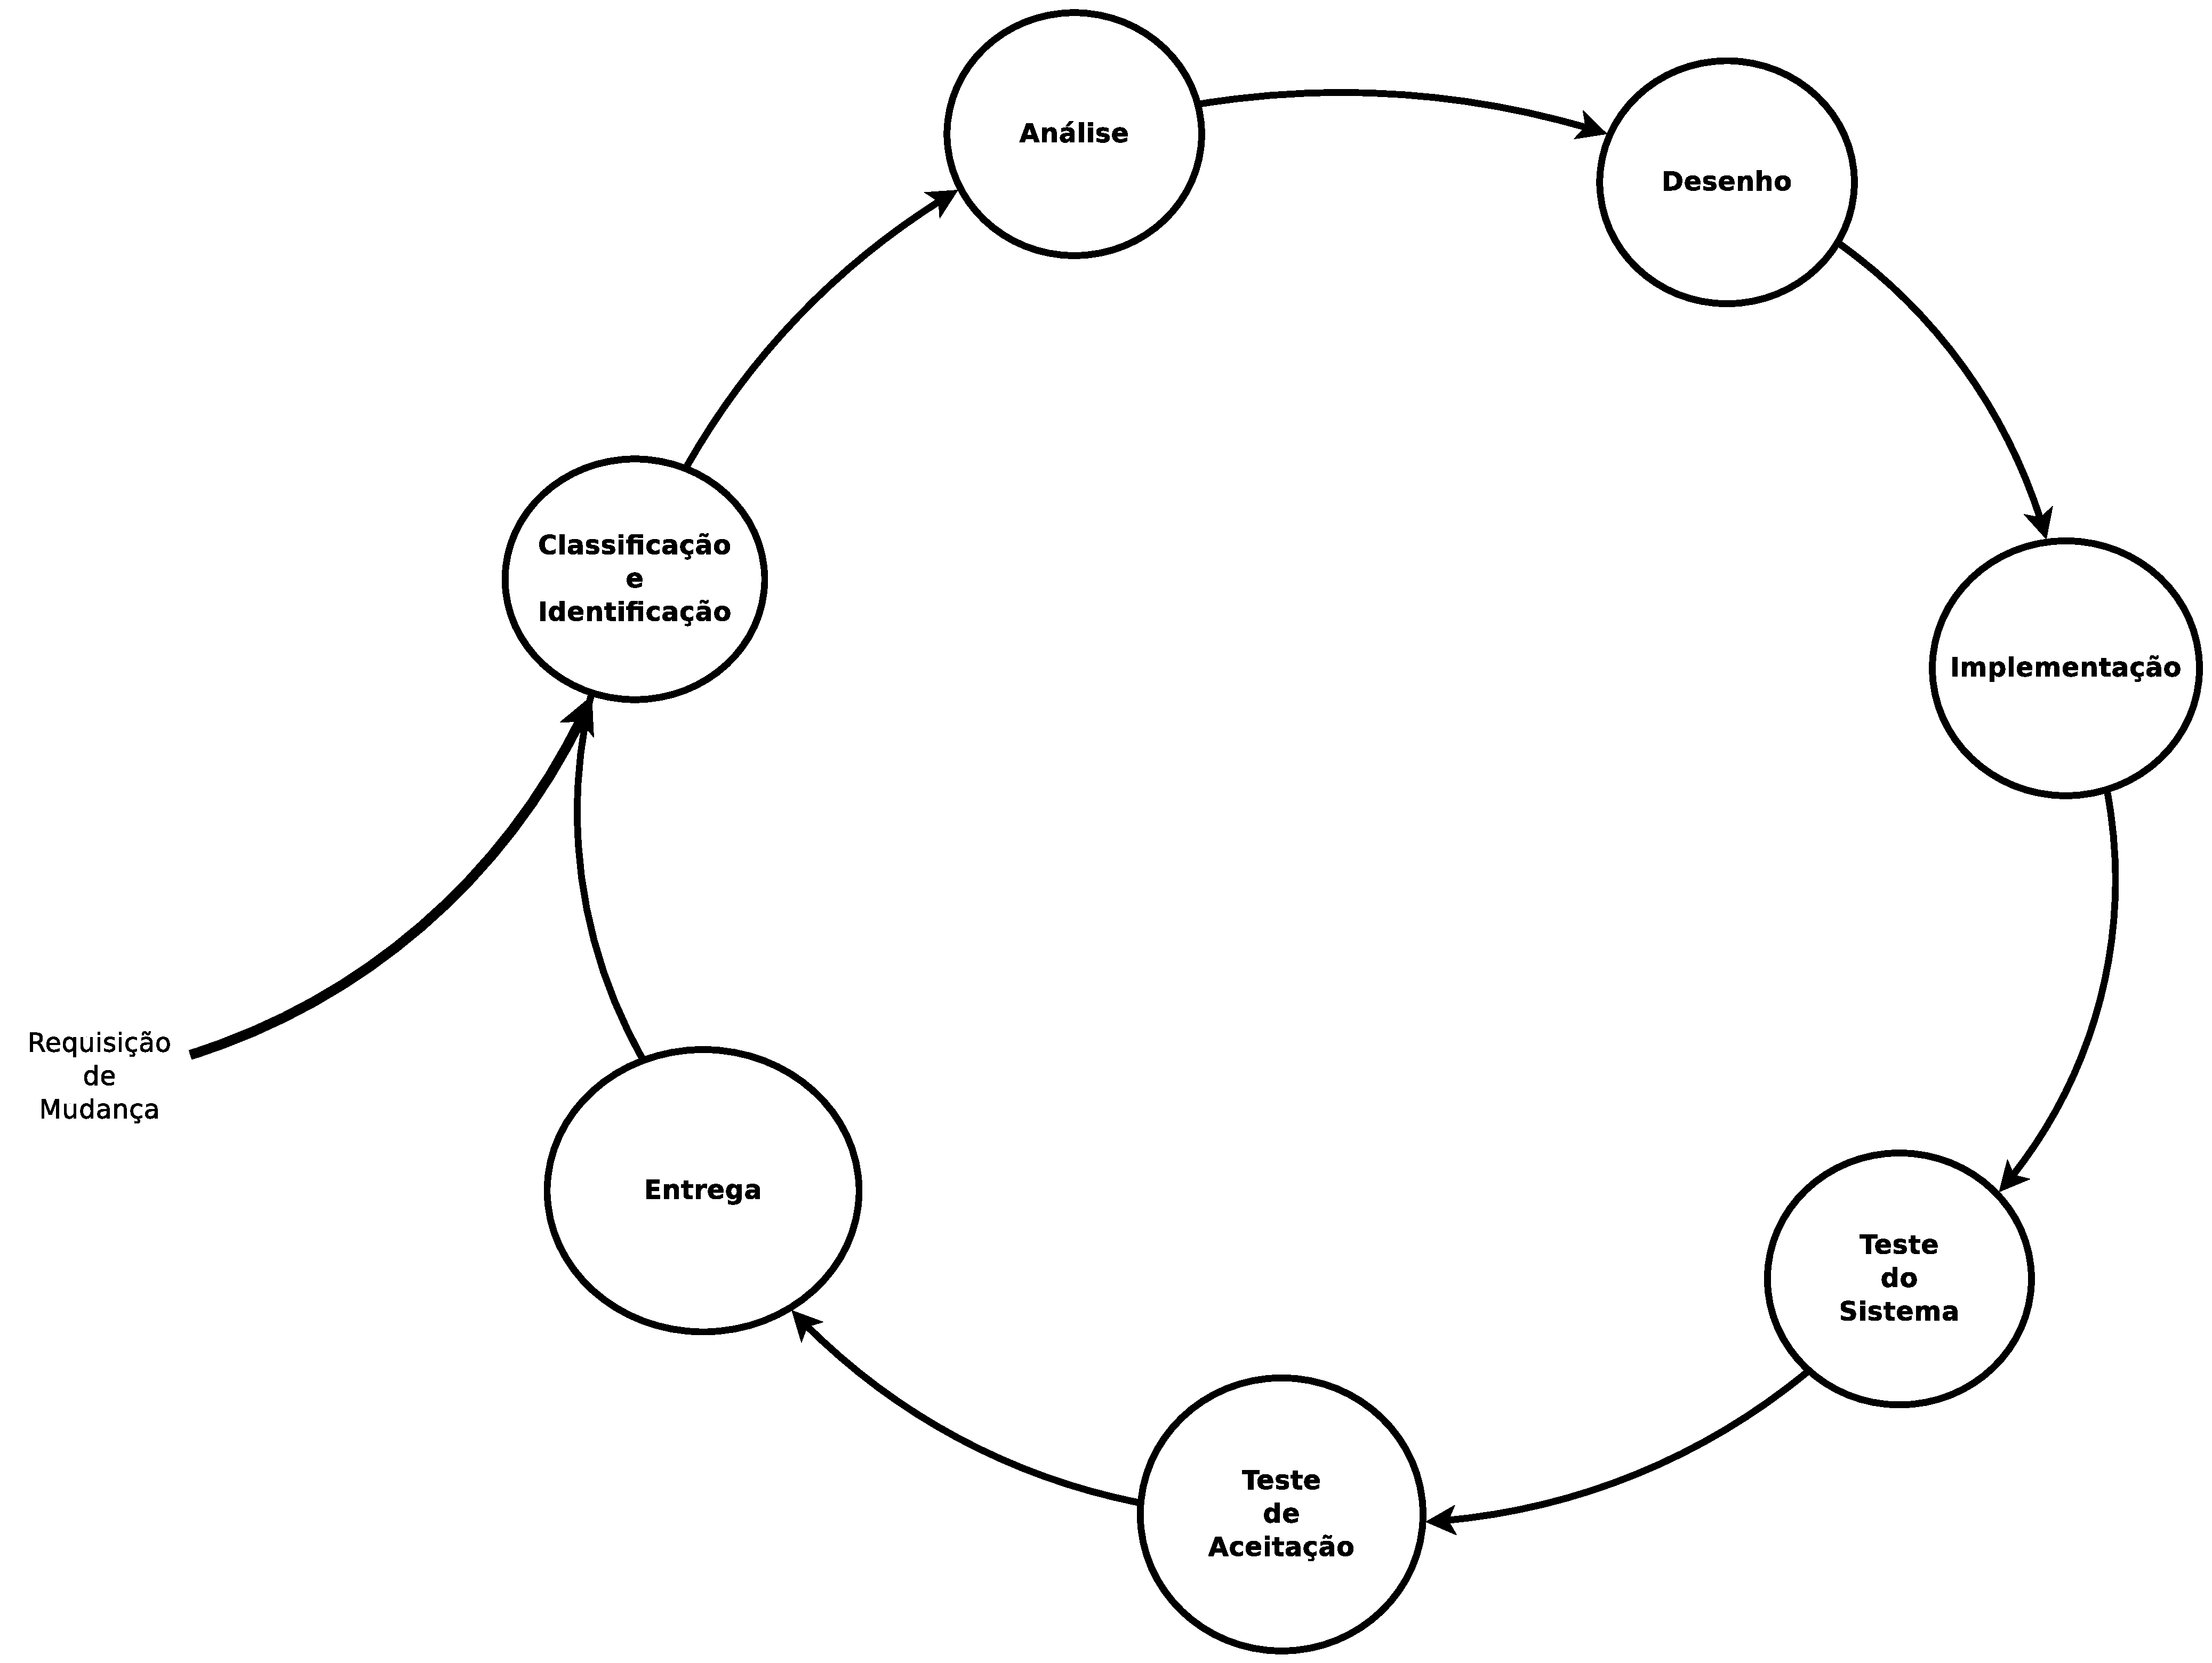
\includegraphics[width=0.9\linewidth]
    {./chapter-manutencao-software-visao-geral/img/ieee_1219_98_processo_manutencao.eps}
	\caption{Processo de Manutenção de
		Software adaptado da norma IEEE~1219~\cite{IEEE1999-Std1219}.}\label{fig:ieee-1219-processo-man-software}
\end{figure}

De maneira relacionada, na ISO/IEC~14764 as atividades que compõem o processo
são similares àquelas propostas na IEEE~1219, exceto pelo fato que elas são
agregadas de uma forma diferente. O processo descrito na ISO/IEC~14764 é
exibido na Figura~\ref{fig:ieee-14764-processo-manutencao}.

\begin{figure}[htpb]
    \centering
    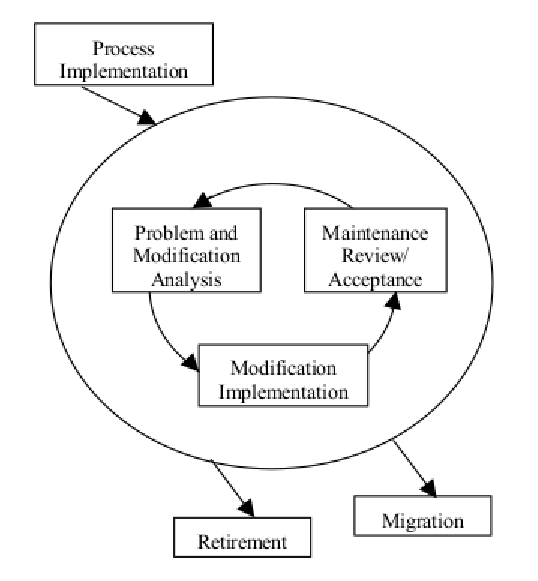
\includegraphics[width=0.9\linewidth]
    {chapter-manutencao-software-visao-geral/img/ieee-14764-processo-manutencao.eps}
    \caption{Processo de Manutenção de Software adaptado da norma
        ISO/IEC~14764~\cite{institute2006norma}.}\label{fig:ieee-14764-processo-manutencao}
\end{figure}

As atividades de manutenção propostas na ISO/IEC~14764 são detalhadas nas
tarefas descritas a seguir:

\begin{itemize}
   	\item Implementação do Processo
   	\item Análise do Problema e da Modificação
    \item Implementação da Modificação
	\item Revisão ou aceitação da Manutenção
   	\item Migração
   	\item Aposentadoria do Software
\end{itemize}

É possível notar que algumas atividades realizadas durante a manutenção de
software são similares a outras presentes no desenvolvimento de software, como
por exemplo, análise de desempenho, codificação, teste e documentação. Outra
atividade comum é o gerenciamento dos requisitos. Nas duas situações os
profissionais responsáveis por controlar os requisitos devem atualizar a
do\-cu\-men\-ta\-ção  por conta de alterações ocorridas no código fonte.

% Por outro lado, certas atividades estão vinculadas apenas ao contexto da
% manutenção de software. O Corpo de Conhecimento em Engenharia de
% Software~\cite{IEEEComputerSociety:2014:GSE:2616205} destaca algumas delas:

% \begin{description}
% 	\item[Compreensão do programa:] atividades necessárias para obter um
% 		conhecimento geral do que um produto de software faz e como as partes
% 		funcionam em conjunto;
%     \item[Aceitação/rejeição de Requisições de Mudança:] as modificações que
%         ultrapassem determinado limiar de tamanho, esforço ou complexidade podem
%         ser rejeitadas pelos mantenedores e redirecionadas para outro
%         desenvolvedor;
% 	\item[Suporte ao usuário:] uma função de suporte para o usuário final que
% 		pode resultar na priorização ou avaliação de esforço das Requisições
% 		de Mudança;
% 	\item[Análise de impacto:] uma técnica para identificar os módulos que
% 		possivelmente são afetados por determinada mudança solicitada;
% 	\item[Contratos de Acordo de Nível de Serviço (\textit{Service Level Agreements
% 		\@-\@ SLA}):] acordos contratuais que descrevem os serviços a serem
% 		realizados pela equipe de manutenção e os objetivos de qualidade do
% 		produto de software.
% \end{description}

\subsubsection{Manutenção de Software na Perspectiva dos Agilistas}\label{sub:manutenção_de_software_com_método_dos_agilistas}

Grande parte da literatura em Manutenção de Software trata de técnicas e
metodologias tradicionais da Engenharia de Software. Todavia, verifica-se a
tendência de que os departamentos dedicados à Manutenção de Software se mostrem
interessados nas metodologias propostas pelos agilistas~\cite{Heeager2015}.  No
momento da elaboração desta dissertação boa parte dos textos de Engenharia de
Software tratam desenvolvimento e manutenção como atividades com natureza
distintas. Todavia, algumas ``práticas ágeis'' podem ser utilizadas em tarefas
de manutenção tais como processo de trabalho iterativo, um maior envolvimento
do cliente, a comunicação face a face e os testes frequentes.

A adoção das práticas dos agilistas na manutenção de software pode apresentar
algumas dificuldades~\cite{1402140}. Entre elas está a adequação das práticas
da organização com as necessidades da equipe de desenvolvimento. Por outro
lado, a adoção de um modelo de manutenção de software usando práticas da
Programação Extrema (\textit{Extreme Programming \@-\@ XP}) apresentou como
resultado melhorias no aprendizado e produtividade da equipe por meio do
aumento da moral, encorajamento e confiança entre os
desenvolvedores~\cite{Choudhari:2014:EIM:2557833.2557845}.

\subsection{Papéis na Manutenção de Software}\label{subsec:man_visao_geral_papeis_na_manutencao_de_software}

As ações realizadas durante a manutenção de um software podem ser desempenhadas
por uma ou mais pessoas. Similarmente ao que ocorre em equipes de
desenvolvimento, cada integrante de uma equipe de manutenção pode desempenhar
um ou mais papéis. Os nomes e as atividades desenvolvidas por cada um pode
variar, contudo, é possível determinar uma classificação que agregue pontos
comuns entre os diferentes papéis. Nesta dissertação, utilizamos a
classificação proposta por Polo e outros~\cite{Polo1999} cujo objetivo é
definir uma estrutura da equipe de manutenção através da identificação de
papéis responsáveis por tarefas. O conjunto de papéis é o resultado da
aplicação da metodologia MANTEMA~\cite{756695} em projetos de software
bancários espanhóis em que o setor de manutenção foi terceirizado
(\textit{outsourcing}). Os autores reforçam que apesar da classificação ter
sido criada em um contexto específico, ela pode ser utilizada para aplicação em
outras situações.

Para esta dissertação removemos os papéis que segundo o nosso entendimento
estão mais vinculados a um contexto de manutenção terceirizada. Além disso,
dividimos o papel ``equipe de manutenção' (\textit{maintenance team}) em
\textit{Desenvolvedor e Analista de Qualidade} por entendermos que são
atribuições comuns a muito dos processos de manutenção existentes. Além disso,
o perfil \textit{Usuário} foi dividido em \textit{Usuário Afetado} e
\textit{Reportador}, especialmente para explicitar as atividades relacionadas à
relatar RMs. O estudo de Polo e outros não explicita o papel responsável pela
atribuição das RMs, contudo, entendemos que em cada equipe de manutenção a
atribuição é realizada de forma adequada. Os papéis que compõem a classificação
utilizadas durante o texto da dissertação estão descritos a seguir:

\paragraph{Usuário Afetado:}
Indivíduo que utiliza o software correspondente à Requisição de Mudanças (RM)
que será relatada. O defeito, a melhoria ou evolução no software, representada
pela RM, estão relacionadas com os desejos e necessidades deste papel.

\paragraph{Reportador:}
Responsável por registrar a RM\@. Em certas situações este papel é desempenhado
tanto pelo usuário do sistema quanto pela equipe de manutenção.

\paragraph{Gerente de Requisição de Mudança (\textit{Maintenance-request
        manager}):} Res\-pon\-sá\-vel por decidir se uma RM será aceita ou
rejeitada. Além disso, ele define qual tipo de manutenção deverá ser aplicada.
Posteriormente cabe ao profissional que cumpre este papel encaminhar a RM para
o Escalonador.

\paragraph{Escalonador (\textit{Scheduler}):}
Deve planejar a fila das RMs que foram aceitas, ou seja, que tenham sido
aprovadas pelo Gerente de Requisição de Mudança.

\paragraph{Desenvolvedor:}
Responsável por realizar as ações que irão solucionar a RM\@.

\paragraph{Analista de Qualidade:}
Tem por responsabilidade avaliar se uma RM solucionada por um Desenvolvedor foi
resolvida de forma correta e dentro dos padrões de qualidade exigidos pelo
projeto.

\paragraph{Chefe da Manutenção (\textit{Head of	Maintenance}):}
Este papel é responsável por definir os padrões e procedimentos que compõem o
processo de manutenção que será utilizado.

Apesar da classificação de papéis derivar de um contexto específico (setor
bancário e empresas com a área de manutenção terceirizada), ela é capaz de
acoplar com alguns tipos de modelos de processo de manutenção existentes na
literatura.

Cabe ressaltar que está fora do escopo deste estudo elaborar uma classificação
dos papeis envolvidos na Manutenção de Software em função de supormos que isto
corresponde a um esforço bem extenso. Nossa ação é identificar alguns dos
papeis e quais são eles, sem com isso, nos envolvermos em uma consolidação
definitiva.

\subsection{Requisição de Mudança}\label{sec:requisicao_de_mudanca}

\subsubsection{Conceitos Básicos}\label{subsec:tipos_de_requisicoes_mudanca}

Uma Requisição de Mudança (RM) corresponde ao registro da informação sobre o
defeito, evolução ou melhoria de um sistema~\cite{tripathy2014software}. De
maneira geral, uma RM pode ser especializada como o \textit{Pedido de Correção}
de uma falha ou o \textit{Pedido de Melhoria} que pode estar relacionado com o
aprimoramento de funcionalidades ou com a melhoria da qualidade do sistema. Esta
visão é apresentada na Figura~\ref{fig:diagrama-classe-requisicao-mudancas}.
Alguns autores utilizam os termos \textit{relato de defeito ou relato de
    melhoria} como sinônimos para a RM\@. Todavia, no escopo desta dissertação,
o relato é um atributo da RM que representa o texto que descreve uma falha ou
pedido de melhoria (vide
Figura~\ref{fig:diagrama-classe-atributos-requisicao-mudancas}).

\begin{figure}[htpb]
	\centering
	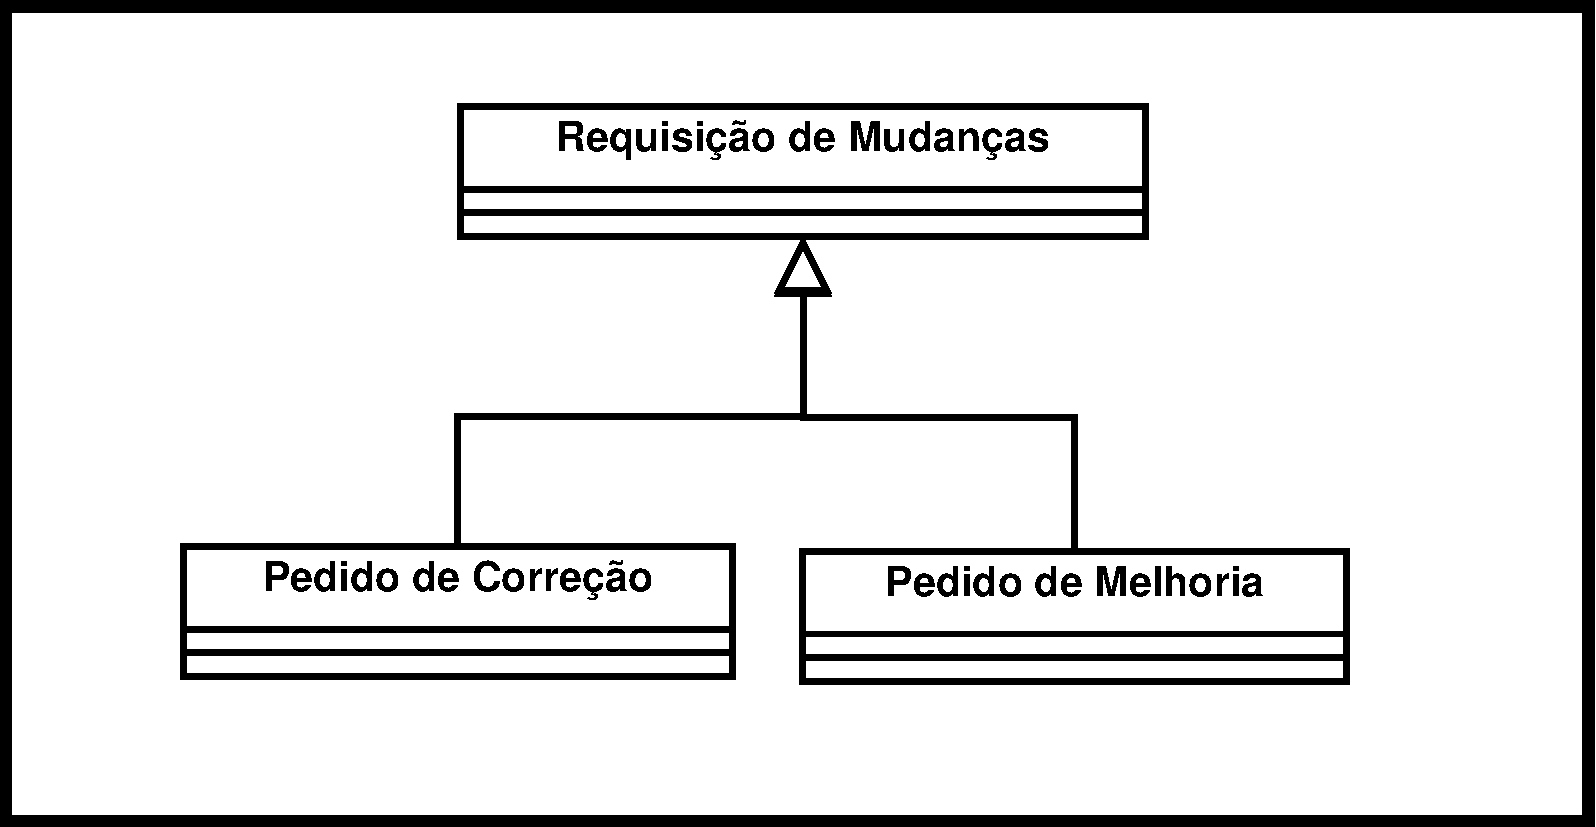
\includegraphics[width=0.5\linewidth]{./chapter-manutencao-software-visao-geral/img/diagrama-classe-conceitual-requisicao-mudancas.pdf}
	\caption{Modelo conceitual de uma Requisição de Mudança.}\label{fig:diagrama-classe-requisicao-mudancas}
\end{figure}

As principais características que compõem uma RM podem ser visualizadas no
modelo exibido na
Figura~\ref{fig:diagrama-classe-atributos-requisicao-mudancas}. Trata-se de uma
adaptação do que foi proposto no trabalho de Singh e
Chaturvedi~\cite{singh2011bug} que descreve um processo genérico de como uma RM
é relatada.

\begin{figure}[htpb]
	\centering
	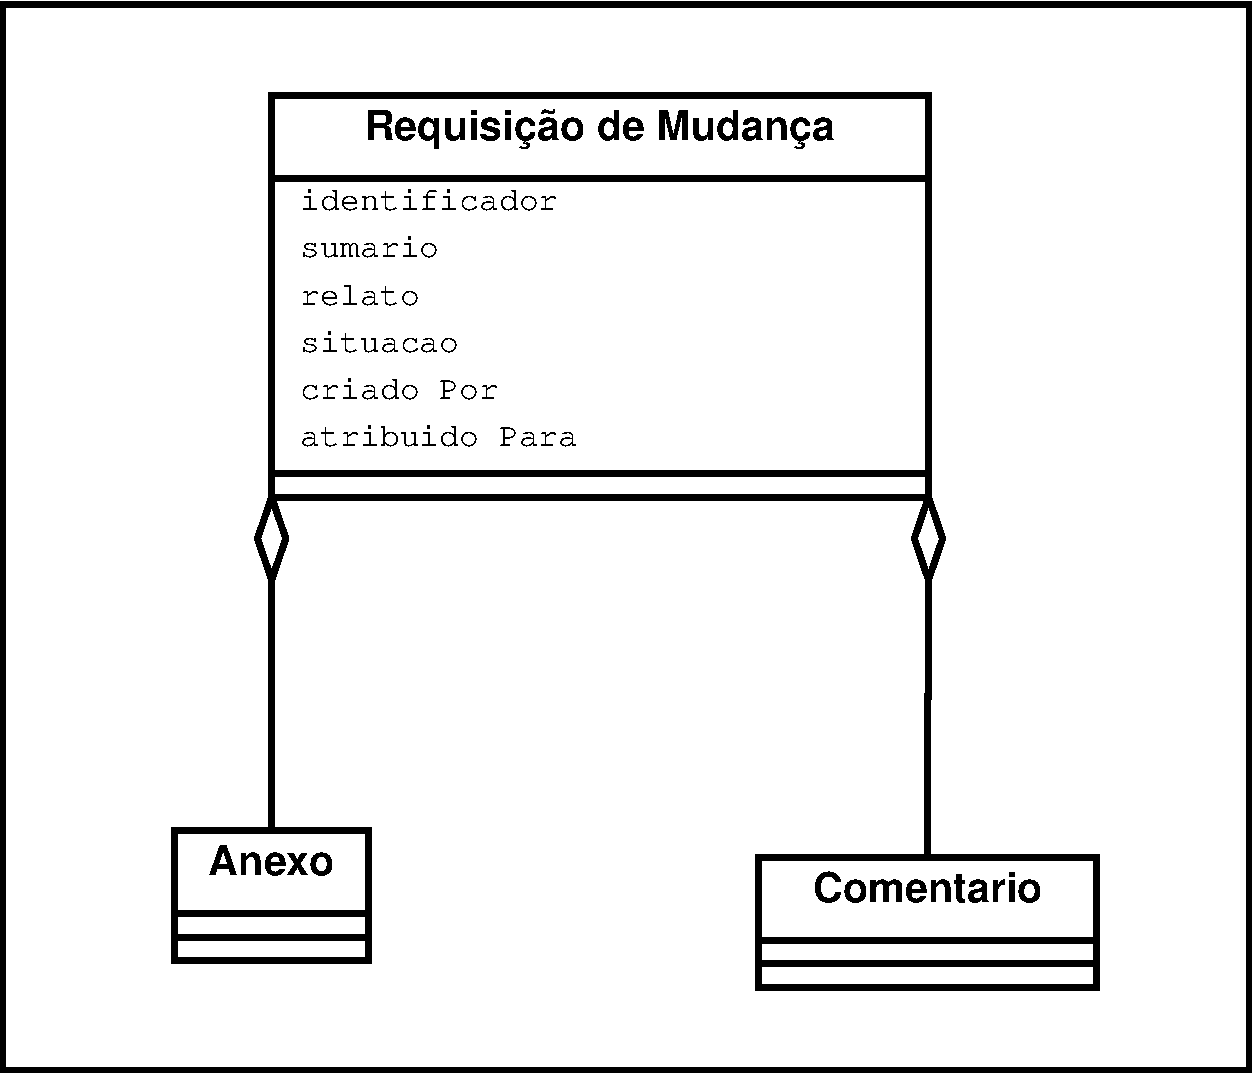
\includegraphics[width=0.5\linewidth]{./chapter-manutencao-software-visao-geral/img/diagrama-classe-atributos-requisicao-mudancas.pdf}
	\caption{Informações que compõem uma RM}\label{fig:diagrama-classe-atributos-requisicao-mudancas}
\end{figure}

Os principais elementos envolvidos no modelo estão detalhados a seguir:

\begin{description}
    \item [Identificador:] Sequência de caracteres, geralmente numérica,  que
        permite distinguir de maneira única uma RM\@.
	\item [Sumário:] Um título ou resumo da RM\@.
    \item [Relato:] Descrição detalhada da RM incluindo ``o que'', ``onde'',
        ``por quê'', ``como'' e ``quando'' a situação relatada ocorreu. A
        mensagem que aparece durante a operação do sistema pode ser incluída,
        bem como a entrada inserida e/ou a saída esperada.
	\item [Situação:] A situação atual de uma RM\@. Representa os diversos
		estados que uma RM possui em seu ciclo de vida. Nesta dissertação
		discutimos brevemente o ciclo de vida de uma RM na
		Subseção~\ref{sub:fluxo_de_trabalho_requisicao_mudanca}.
    \item [Criado Por:] Nome da pessoa ou um identificador previamente registrado
        no sistema de quem criou a RM\@.
    \item [Atribuído Para:] A RM pode ser atribuída a uma pessoa específica
        caso ela seja capaz de resolvê-la, caso contrário, a RM será atribuída
        para alguém que possui o papel de definir o desenvolvedor mais apto
        para solucioná-la.
    \item [Anexo:] Refere-se à informação em formato diferente de texto e que
        pode ser incluída na RM\@. Por exemplo, casos de teste, capturas de
        tela, e cadeia de registros de ativação (\textit{stack trace}).
    \item [Comentário:] Registra o histórico de discussões realizadas durante o
        processo de solução da RM\@\footnote{O conceito de solução bem como de
            outros relacionados ao ciclo de vida de uma RM estão descritos com
            maiores detalhes na
            Seção~\ref{sub:fluxo_de_trabalho_requisicao_mudanca}}.
\end{description}

Conforme pode ser observado na
Figura~\ref{fig:diagrama-classe-atributos-requisicao-mudancas} os atributos
\textit{Comentário} e \textit{Anexo} foram modelados como uma agregação, dando
aos mesmos um caráter multivalorado. Esta escolha foi intencional para salientar
que uma RM pode conter diversos anexos ou comentários. No caso dos comentários
esta característica é ainda mais relevante tendo em vista que eles são
realizados durante o processo de solução de uma RM\@. A partir do conjunto de
comentários é possível coletar informações relevantes para a manutenção do
software e que podem ser utilizadas para solucionar futuras RMs.

Os atributos que compõem uma RM podem variar dependendo de fatores como a
ferramenta utilizada para o gerenciamento, o projeto e a equipe de manutenção.
Esses campos fornecem uma variedade de metadados descritivos tais como
\textit{importância, prioridade, gravidade, componente, e
    produto}~\cite{zhang2016literature}. Em alguns casos a RM pode conter um
campo de modo a relacioná-la com outra já existente na base de dados. Este tipo
de vínculo é importante para minimizar problemas da gestão das RMs, como por
exemplo, a duplicação discutida na
Subseção~\ref{ssub:problemas_relacionadas_rm}. A Figura~\ref{fig:rm-exemplo}
exibe um exemplo de uma RM contendo os elementos básicos descritos no modelo
proposto na Figura~\ref{fig:diagrama-classe-atributos-requisicao-mudancas}.

\begin{figure}[htpb]
	\centering
	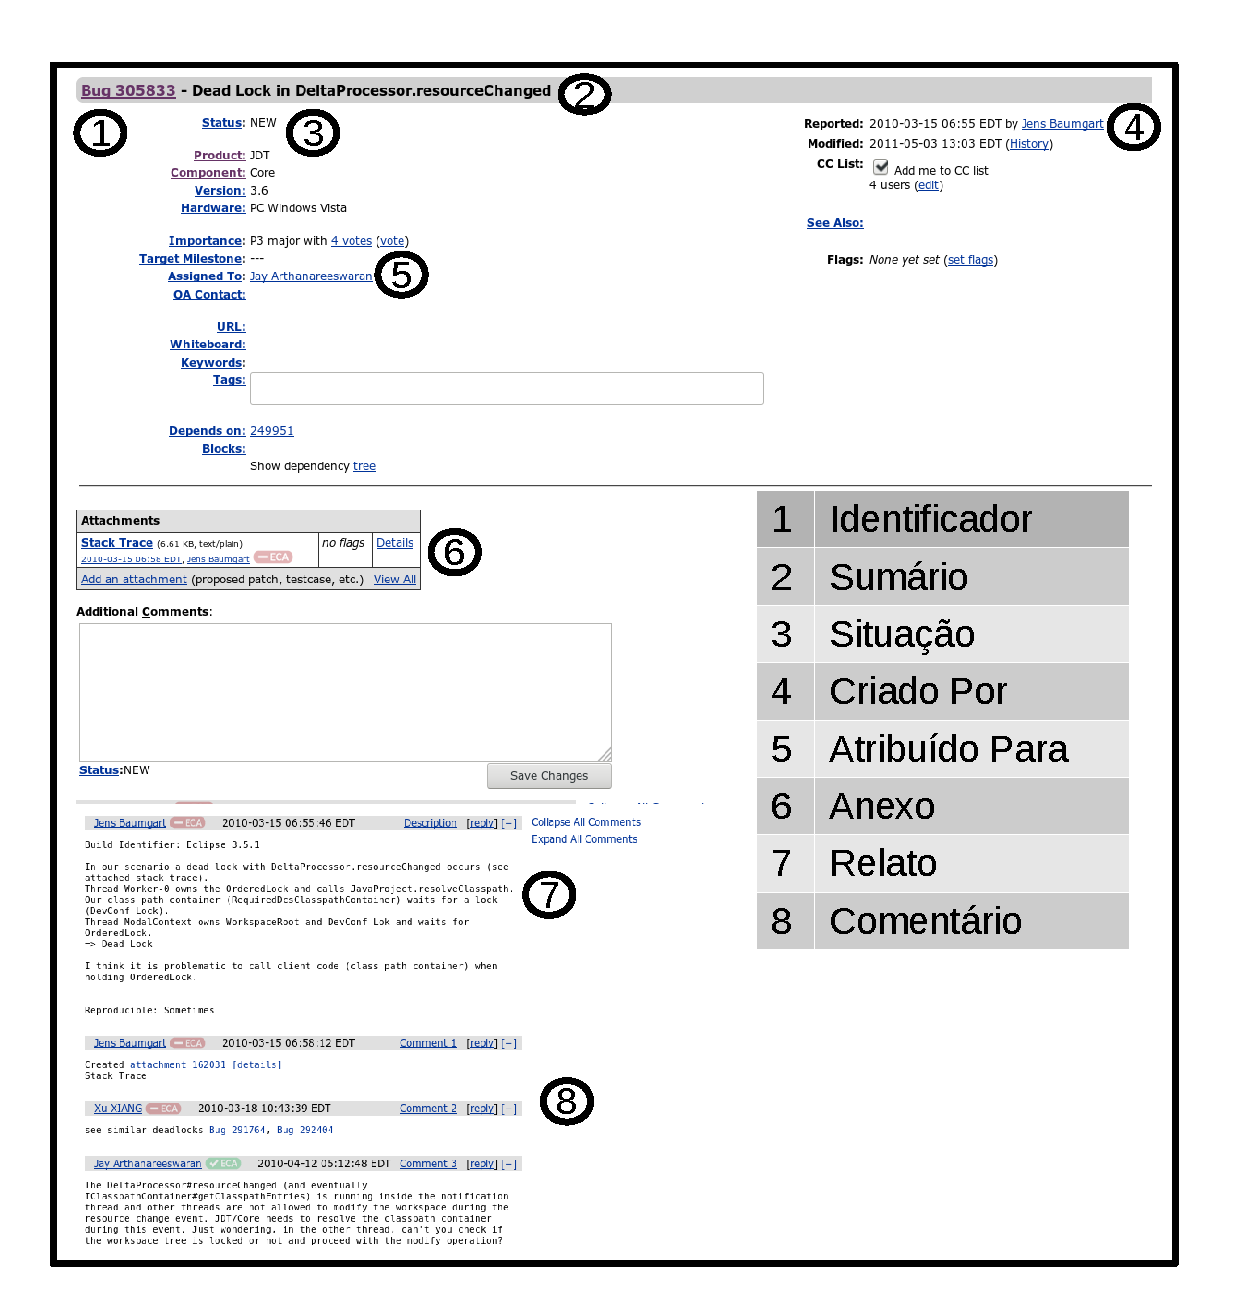
\includegraphics[width=0.9\linewidth]{./chapter-manutencao-software-visao-geral/img/rm-exemplo.pdf}
	\caption{Um exemplo de uma RM do Projeto Eclipse}\label{fig:rm-exemplo}
\end{figure}

Em síntese, apesar das diferentes nomenclaturas existentes na literatura
(demanda, bug, defeito, bilhete, tíquete, requisição de modificação, solicitação
de modificação, relato de problema) uma Requisição de Mudança representa uma
descrição, independente da estrutura, que visa gerar a manutenção ou evolução do
software. A manutenção ou evolução estão relacionados com o reparo de uma falha
ou com um desejo ou necessidade do usuário do software. Nesta dissertação
procuramos ficar aderentes ao termo ``Requisição de Mudança'' e sua sigla
\textit{RM}.

\subsubsection{Ciclo de Vida de uma Requisição de Mudança}\label{sub:fluxo_de_trabalho_requisicao_mudanca}

Uma RM descreve os desejos e necessidades dos usuários de como um sistema deve
operar. Quando uma RM é relatada pelo menos dois fatores devem ser levados em
conta~\cite{tripathy2014software}:

\begin{itemize}
    \item \textit{Corretude da RM:} uma RM deve ser descrita de forma não
        ambígua tal que seja fácil revisá-la afim de determinar sua corretude.
        O ``formulário'', que corresponde aos campos que devem ser preenchidos
        na RM, é a chave para efetiva interação entre desenvolvedores e
        usuários. O formulário, neste sentido, documenta informações essenciais
        sobre mudanças no software, hardware e documentação.
   \item \textit{Comunicação clara das RMs para as partes
           interessadas\footnote{Na
               Seção~\ref{subsec:man_visao_geral_papeis_na_manutencao_de_software}
               discutimos em maior detalhe as diferentes partes interessadas
               no contexto da manutenção de software.}}: as RMs necessitam ser
       claramente comunicadas para as partes interessadas. O resultado de
       avaliar de maneira distinta uma RM pode ser contra-produtivo:
       \textit{(i)} a equipe que realiza mudanças no sistema e a equipe que
       executa testes podem ter visões contraditórias sobre a qualidade do
       software; \textit{(ii)} O sistema alterado pode não atender às
       necessidades e desejos dos usuários finais.
\end{itemize}

No caminho entre sua criação e solução uma RM possui diferentes estágios. O
ciclo de vida de uma RM é ilustrado através do diagrama de estados da
Figura~\ref{fig:diagrama-estado-rm}. Nele uma RM inicia como \textit{Submetida
    (Submit)} e vai sendo modificada até alcançar o estado \textit{Fechada
    (Closed)}, em que é considerada como solucionada. Neste caminho o conjunto
de fatores que resultou na necessidade de relatar a RM pode não mais existir.
Neste caso, ela é alterada para o estado \textit{Rejeitada (Decline)}.

Existe um aspecto importante do ciclo de vida de uma RM não abordado na
discussão apresentada por Tripathy e Naik. Em teoria uma RM poderia ter novos
estados: ``Reaberta'', quando um usuário ou outro membro da equipe de
manutenção entende que ela não foi solucionada; ``Relacionada'', quando uma
nova RM é na realidade uma sucessora ou possui algum tipo de relação com outra
RM anteriormente registrada.

\begin{figure}[htpb]
	\centering
    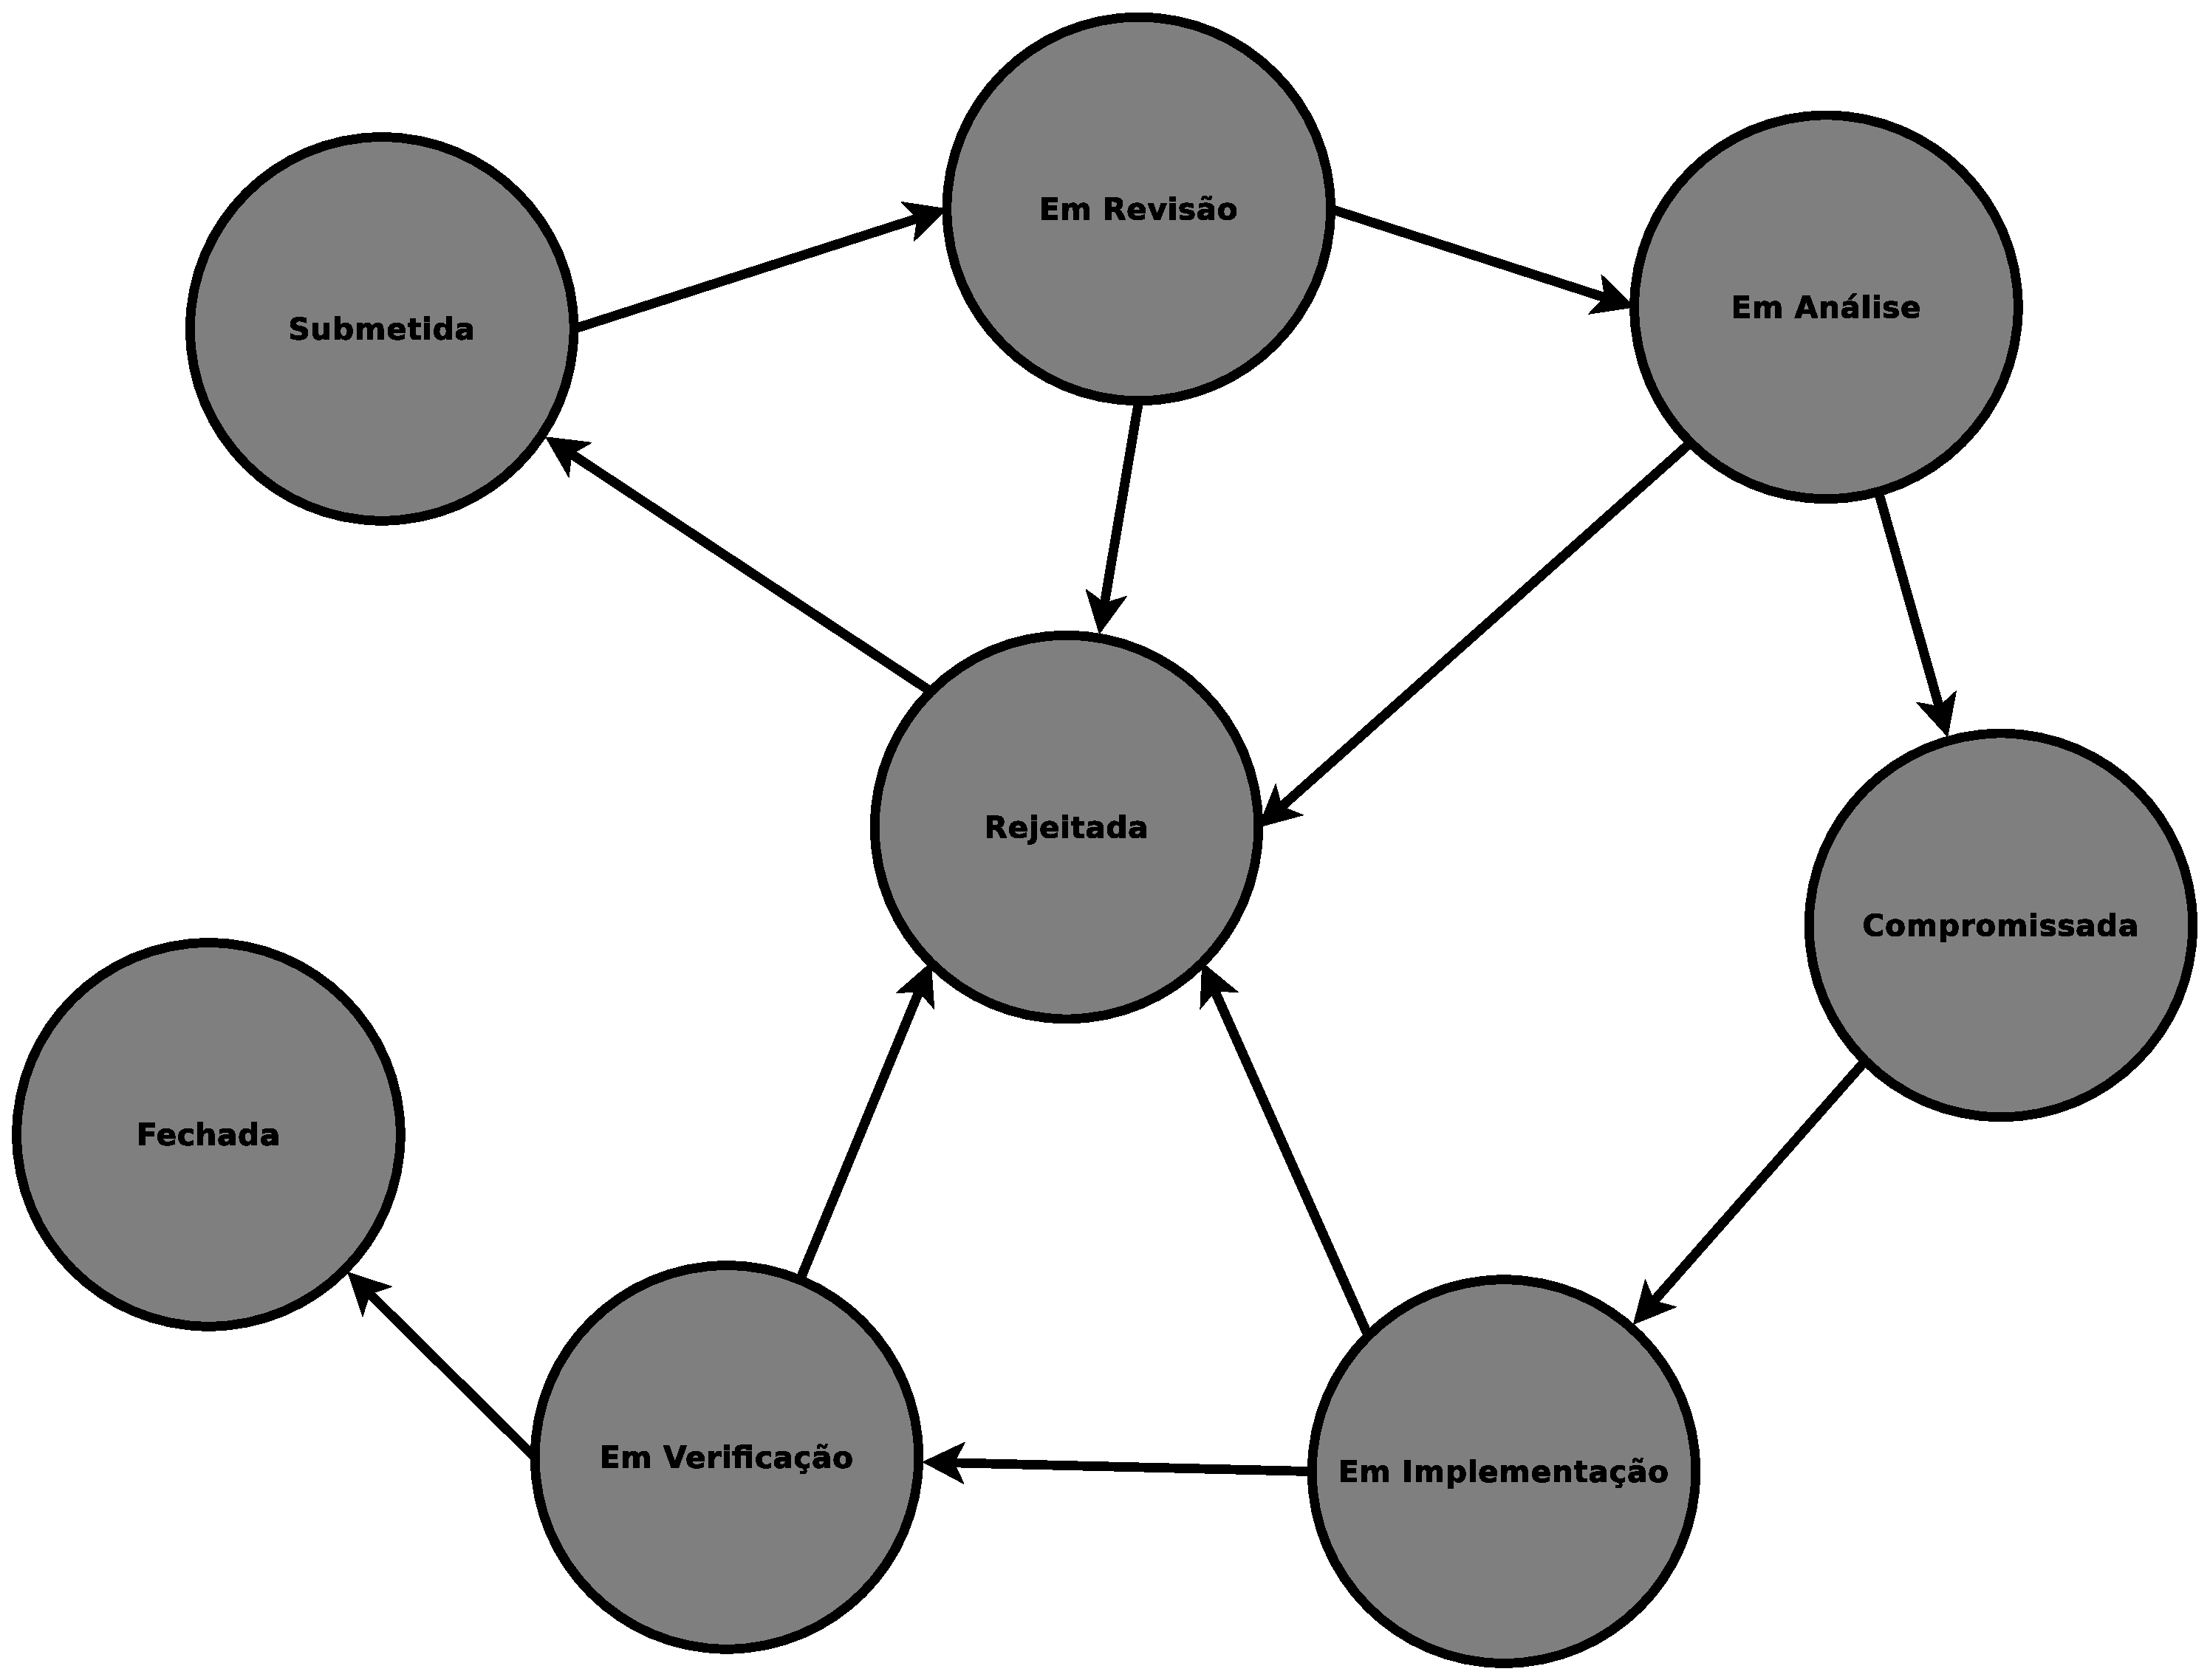
\includegraphics[width=0.7\linewidth]{./chapter-manutencao-software-visao-geral/img/diagrama-estado-rm.eps}
	\caption{Diagrama de estados de uma RM\@. Adaptado
		de~\cite{tripathy2014software}}\label{fig:diagrama-estado-rm}
\end{figure}

A seguir apresentamos as características dos estados do ciclo de vida de uma
RM~\cite{tripathy2014software}. Para cada estado pode haver mais de um papel
responsável pelas ações executadas. Também pode ocorrer que uma mesma pessoa
desempenhe diferentes papéis neste processo, conforme discutido na
Seção~\ref{subsec:man_visao_geral_papeis_na_manutencao_de_software}.

\paragraph{Submetida (\textit{Submit}):}\label{par:submetida)}

Este é o estado inicial de uma RM criada. Geralmente são os usuários do sistema
a fonte primária das RMs nesta situação. Com base no nível de prioridade, ela é
movida de \textit{Submetida} para \textit{Em Revisão}. Normalmente cabe ao
\textit{Gerente de Requisição de Mudança} a responsabilidade da manipulação
inicial das RMs. Neste instante ele se torna o ``dono'' das mesmas.

\paragraph{Em Revisão (\textit{Review}):}\label{par:em_revisao}
Normalmente, cabe ao \textit{Gerente de Requisição de Mudanças} manipular as
RMs no estado \textit{Em Revisão} através das seguintes atividades:

\begin{itemize}
    \item Verificar se a RM submetida recentemente é idêntica a outra já
        existente. Se ela é identificada como duplicada o estado da mesma é
        alterado para \textit{Rejeitada}. Neste caso, uma breve explicação e
        algum tipo de ligação para a original são inseridos nos comentários da
        RM\@.
	\item Aceitar o nível de prioridade atribuído para a RM ou alterá-lo.
	\item Determinar o nível de severidade da RM\@: normal ou crítico.
\end{itemize}

Caso as atividades descritas anteriormente não possam ser re\-a\-li\-za\-das, a
RM é movida para o estado \textit{Em análise}.

\paragraph{Em Análise (\textit{Analysis}):}\label{par:em_analise}

Neste estágio uma análise de impacto é conduzida para entender o que foi
solicitado na RM e estimar o tempo necessário para implementá-la. Caso não seja
possível ou desejável atendê-la a situação é alterada para \textit{Rejeitada}.
Caso contrário, a RM é movida para estado \textit{Compromissada (Commit)}.

\paragraph{Compromissada (\textit{Commit}):}\label{par:commit}

A RM no estado \textit{Compromissada} não foi atendida, mas se encontra no
planejamento do projeto de modo a estar em uma próxima versão do produto. As RMs
neste estado são responsabilidade de um \textit{Gerente de Requisição de
    Mudança}. Algumas RMs podem ser incluídas em futuras versões do sistema após
acordo com as demais partes interessadas.

\paragraph{Em Implementação (\textit{Implement}):}\label{par:em_implementacao}

No estágio de \textit{Em Implementação} diferentes cenários podem ocorrer:

\begin{itemize}
	\item A RM pode ser rejeitada caso sua implementação não seja factível.
    \item Caso a RM seja possível de implementar, os desenvolvedores realizam a
        codificação e os testes. Após o desenvolvimento ser finalizado a RM é
        movida de \textit{Em Implementação} para \textit{Em verificação}.
\end{itemize}

\paragraph{Em Verificação (\textit{Verification}):}\label{par:em_verificacao}

No estado de verificação as atividades são controladas pelo \textit{Analista de
Qualidade}. Dentre os métodos de verificação temos demonstrações, análises,
inspeções e testes.

\paragraph{Fechada (\textit{Closed}):}\label{par:fechada}

Após a verificação de que a RM foi atendida, ela é movida de \textit{Em
    verificação} para \textit{Fechada}. Esta ação é realizada pelo
\textit{Analista de Qualidade} que é o ``proprietário'' da RM durante o estado
de \textit{Em Verificação}. Nesta dissertação, quando referenciamos ao último
estágio do ciclo de vida da RM, utilizaremos o termo ``Solução da RM'' para
representar a situação em que a falha relatada ou a melhoria solicitada é
entendida, por algum membro das partes interessadas, como atendida.

\paragraph{Rejeitada (\textit{Decline}):}\label{par:rejeitada}

Uma RM pode ser rejeitada caso ela seja considerada sem impacto relevante no
sistema, não seja possível tecnicamente realizar o que foi solicitado na RM\@ ou
a equipe de qualidade conclui que as mudanças no software para atender à RM não
podem ser satisfatoriamente verificadas.

O modelo de ciclo de vida discutido por Tripathy e Naik possui foco em
organizações que possuem uma área exclusivamente dedicada à manutenção de
software. Em outros contextos, como por exemplo em projetos de código aberto, o
processo de modificação dos estados de uma RM pode ser diferente. No trabalho de
Ihara e outros~\cite{ihara2009analysis} foi conduzido um estudo de caso nos
projetos Firefox e Apache e um dos resultados foi o diagrama apresentado na
Figura~\ref{fig:diagrama-estado-rm-codigo-aberto} que representa o processo de
modificação de uma RM\@.

\begin{figure}[htpb]
	\centering
    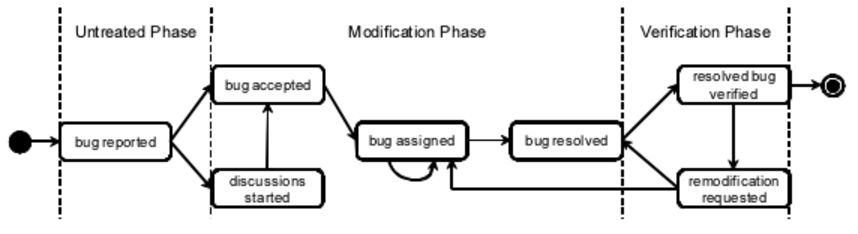
\includegraphics[width=0.8\linewidth]{./chapter-manutencao-software-visao-geral/img/diagrama-estado-rm-codigo-aberto.pdf}
    \caption{Um processo de modificação de uma RM utilizando uma FGRM\@.
        Extraído de~\cite{ihara2009analysis}}\label{fig:diagrama-estado-rm-codigo-aberto}
\end{figure}

Os autores ponderam que apesar de haver diferentes estados e transições em
diferentes projetos, o diagrama é capaz de representar de maneira geral o
processo de transição de uma RM\@. O processo é composto de três fases
diferentes: \textit{não tratada (untreated), modificação (modification) e
    verificação (verification)}.

A fase \textit{não tratada} foca em um subprocesso em que as RMs são relatadas,
todavia, não foram aceitas ou atribuídas a algum membro da equipe. A fase de
\textit{modificação} é um subprocesso em que as RMs são efetivamente
modificadas. Nesta fase uma RM é aceita e posteriormente atribuída a algum
desenvolvedor. Caso o pedido da RM não possa ser atendido ela é
\textit{rejeitada}. A fase de \textit{verificação} é o subprocesso em que
membros com a responsabilidade de garantia da qualidade verificam se as RMs
modificadas foram efetivamente solucionadas. Caso uma RM modificada por um
desenvolvedor não seja verificada, ela poderia não ser reconhecida como fechada
(\textit{closed}).

É possível relacionar o modelo descrito por Tripathy e Naik e aquele proposto
por Ihara e outros. Em ambos é possível identificar fases em que uma RM é
relatada, analisada e verificada. Além disso, os modelos discriminam situações
em que o pedido descrito na RM não é capaz de ser realizado. Nesta dissertação
utilizamos de forma geral o modelo proposto por Ihara e outros.

\subsubsection{Problemas e Desafios do Gerenciamento das RMs}\label{ssub:problemas_relacionadas_rm}

A seguir discutimos alguns dos problemas e desafios do gerenciamento de RMs
discutidos na literatura.

\paragraph{Localização do Problema:}

A tarefa de encontrar a origem de uma falha de software em boa parte das vezes é
complexa e consome muito tempo. O estudo de Thung e outros afirma que na faixa
de 84 a 93\% de problemas em software afetam entre 1 e 2 arquivos de
código-fonte~\cite{thung2012faults}. Apesar da pequena quantidade de arquivos
afetados, identificar em quais deles o problema reside (buggy files) é uma
tarefa árdua~\cite{Thung:2014:BIT:2635868.2661678}.

Os pesquisadores vêm propondo abordagens baseadas em Recuperação da Informação
para localizar o arquivo que contém uma falha com base no texto do relato de
uma RM\@. Nesse tipo de abordagem existe a tentativa de encontrar um elo entre
o texto do relato e os arquivos que podem estar relacionados com a solução do
problema~\cite{Wong:2014:BBF:2705615.2706096}.

\paragraph{Dificuldade na Visualização das Informações das RMs:}

Uma tomada de decisão deve ser subsidiada por informações corretas. Este fato
não é diferente na manutenção e desenvolvimento de software. Pouco se sabe sobre
o comportamento evolutivo, o tempo de vida, distribuição e estabilidade dos
problemas reportados nas FGRMs~\cite{hora2012bug}. Este problema é reforçado
pela forma como as FGRMs armazenam os dados das RMs. Em geral, essas ferramentas
exibem informações sobre as RMs de forma textual, o que não é apenas complicado
para navegar, mas também dificulta a compreensão dos problemas do
software~\cite{dal2014bug}. Por esta razão estudos estão sendo realizados de
modo a propor novas formas de visualização da informação contida nas
RMs~\cite{takama2013application,hora2012bug}.

\paragraph{Baixa Qualidade do Relato:}

Durante o processo de solução de uma RM a reprodução manual das falhas
reportadas é demorada e tediosa. Os desenvolvedores tentam reproduzir problemas
usando a informação contida nas RMs que muitas vezes está
incompleta~\cite{White:2015:GRR:2820282.2820291}. Em algumas situações, para
obter os dados que necessita, o desenvolvedor deve registrar um comentário para
que o responsável do relato inclua as informações necessárias~\cite{5070993}. A
melhoria da qualidade do relato pode implicar na redução do custo do processo de
garantia de qualidade bem como aumentar a confiabilidade do software com a
redução gradativa de falhas~\cite{Tu:2014:MQI:2677832.2677844}.

\paragraph{Identificação de RMs Duplicadas:}

O processo de identificação de RMs Duplicadas consiste em avaliar se determinado
relato de uma RM trata do mesmo assunto tratado no relato de outra RM\@. Quando
uma RM é identificada como duplicada ela deveria ser relacionada com a sua
``cópia''. Uma delas é definida como RM Mestre e as demais RMs Filhas.
Geralmente a Mestre é aquela que foi primeiramente incluída no repositório de
erros. Alguns estudos revelam que entre 10\% e 30\% das RMs podem ser
classificadas como
duplicadas~\cite{anvik2005coping,cavalcanti2013bug,Runeson:2007:DDD:1248820.1248882}.
Por conta do grande número de RMs repetidas uma das soluções é durante o
processo de atribuição a análise seja realizada de forma manual com objetivo de
evitar que elas cheguem aos desenvolvedores~\cite{anvik2005coping}. Em alguns
casos esta solução não é viável. O processo de identificação de RMs duplicadas
requer: \textit{(i)} um prévio conhecimento do conjunto de relatos existentes
anteriormente no projeto; \textit{(ii)} a busca manual em toda base de dados da
FGRM~\cite{banerjee2012automated,
    Lerch:2013:FDY:2495256.2495763,hindle2016contextual}. Ambas as estratégias
consomem tempo e não garantem que falsos positivos não possam
ocorrer~\cite{kaushik2012comparative}. Os falsos positivos podem ainda
acarretar na desconsideração de problemas relevantes.

\paragraph{Atribuição da RM:}

O processo de atribuição de RMs tem como objetivo encontrar o desenvolvedor
mais capacitado para manipular uma dada RM~\cite{cavalcanti2014challenges}.
Existe a premissa de que a escolha do desenvolvedor apropriado é crucial para
obter em menor tempo a so\-lu\-ção da RM~\cite{di2002approach}. Estudos também
discutem que o processo de atribuição deve considerar fatores tais como a carga
de trabalho do desenvolvedor e a prioridade da RM, dentre
outros~\cite{aljarah2011selecting}.

\paragraph{Classificação da RM:}

Independentemente do tipo e tamanho de um projeto é importante determinar qual
tipo de manutenção deverá ser realizada para cada RM que é criada. Geralmente
este tipo de classificação é feita com base no texto que corresponde ao relato
da RM\@. A diversidade de categorias pode tornar a tarefa complexa pelo fato de
que em muitos casos não é fácil determinar os limites entre os
tipos~\cite{antoniol2008bug}. Por exemplo, a uma classificação incorreta de um
defeito que na verdade trata-se de uma melhoria pode acarretar em atrasos no
projeto~\cite{cavalcanti2014challenges}. A principal atividade associada é a
triagem de RMs que tem como objetivo revisar uma lista de RMs para determinar
aquelas que necessitam ser acompanhadas ou priorizadas.

\paragraph{Estimativa de Esforço da RM:}

A gerência de custo e de esforço de um projeto de manutenção passa pelo
controle do esforço necessário para solucionar suas RMs. Os estudos que
discutem o esforço para solução de uma RM utilizam três formas de
estimativa~\cite{cavalcanti2014challenges}: determinar o tempo para solucionar
novas RMs; definir os artefatos que são impactados por determinada RM (Análise
de Impacto); prever o número de novas RMs que poderão fazer parte do projeto. A
literatura sobre análise de impacto é bastante abrangente e pode envolver o
estudo de artefatos tais como documentos de requisitos e arquiteturas de
softwares, código fonte, registros (\textit{logs}) de teste e assim por
diante~\cite{cavalcanti2014challenges}. Apesar da inerente imprecisão deste
tipo de trabalho é importante salientar que a estimativa de esforço de RMs é
importante para a gestão de projetos de manutenção porque ajuda alocar o
recurso disponível de forma mais
eficiente~\cite{Bhattacharya:2011:BTP:1985441.1985472} e melhorar a previsão do
custo necessário para o lançamento de futuras versões do
sistema~\cite{Vijayakumar2014}.

\paragraph{Recomendação de RMs:}

Em algumas equipes, um membro experiente geralmente ensina os recém-chegados o
que eles precisam fazer para solucionar uma RM\@. Todavia, alocar um membro
experiente de uma equipe por um longo tempo para ensinar um novato nem sempre é
possível ou desejável. A premissa é que o mentor poderia ser mais útil fazendo
tarefas mais importantes~\cite{malheiros2012source}. Por exemplo, quando um novo
desenvolvedor entra no projeto seria interessante que ele resolvesse as RMs que
tivessem um menor nível de dificuldade. Posteriormente, quando o desenvolvedor
ganhasse mais experiência, poderia aumentar o grau de dificuldade das RMs que
ele deve tratar. Este tipo de situação ocorre com certa frequência em projetos
de código aberto, em que a contribuição de desenvolvedores externos ao projeto é
fundamental. No entanto, encontrar um defeito apropriado ao nível de
conhecimento do desenvolvedor, bem como a correção apropriada para o mesmo
requer uma boa compreensão do projeto~\cite{Wang2011bug}.

Para facilitar a inclusão de novos desenvolvedores alguns estudos vêm se
dedicando ao desenvolvimento de sistemas de recomendação de
RMs~\cite{malheiros2012source, Wang2011bug}. Estes sistemas podem ajudar o
recém-chegado a solucionar uma RM mediante a apresentação do código fonte
potencialmente relevante~\cite{malheiros2012source}.

\section{As Ferramentas de Gerenciamento de Requisições de Mudança (FGRM)}\label{sec:ferramentas_de_gerenciamento_requisicoes_de_mudanca}

As RMs são controladas por uma FGRM na forma de um fluxo de trabalho de modo a
identificar, descrever e controlar a sua situação. Em geral, os objetivos de um
projeto em adotar uma FGRM para gerenciar suas RMs são os
seguintes~\cite{tripathy2014software}:

\begin{itemize}
    \item Disponibilizar um método comum para a comunicação entre as partes
        interessadas.
	\item Identificar de forma única e rastrear a situação de cada RM\@. Esta
		característica simplifica o processo de relatar uma RM e fornece um
		melhor controle sobre as mudanças.
    \item Manter uma base de dados sobre todas as mudanças no sistema. Esta
        informação pode ser utilizada para monitoramento e métricas de medição.
\end{itemize}

No momento em que os trabalhos desta dissertação estavam sendo desenvolvidos,
alguns estudos discutiam o fato de que as FGRMs não apenas ajudam as
organizações a gerenciar, atribuir, controlar, resolver e arquivar as
RMs~\cite{Bertram:2010:CCB:1718918.1718972}.  Em alguns casos, este tipo de
ferramenta se tornou o ponto focal para comunicação e coordenação para diversas
partes interessadas, dentro e além da equipe de manutenção. As FGRMs servem
como um repositório central para monitorar o progresso das ações dos
mantenedores associadas a uma RM, para solicitar informações adicionais da
pessoa responsável por redigir a requisição e o ponto de discussão para
potenciais soluções de um defeito (bug)~\cite{zimmermann2009improving}.

Em projetos de código aberto, as FGRMs são um importante espaço onde a equipe de
desenvolvimento interage com a comunidade. Como consequência é possível observar
o fenômeno da participação dos usuários no processo de solução da RM:\@ eles não
apenas submetem a RM, mas também participam da discussão da solução. Desta
forma, o usuário final ajuda nas decisões sobre a direção futura do produto de
software~\cite{breu2010information}.

\subsection{Modelo Conceitual do Contexto das FGRMs}\label{sub:espectro_funcionalidades_fgrm}

As FGRMs têm características as vezes distintas e têm sido usadas em diferentes
contextos, apesar disso é possível encontrar atributos comuns que permitem a
compilação de um modelo das FGRMs e de seu contexto. A construção de um modelo
conceitual do contexto das FGRM pode ajudar em discussões posteriores.
Acreditamos que o esforço para a criação de um modelo conceitual para FGRMs e
seu contexto é bem extenso. Conforme discutido na Conclusão desta dissertação
percebemos que organizar de maneira consistente e abrangente as FGRMs e seu
contexto exigiria um esforço além de nossa disponibilidade e aqui apenas
itemizamos alguns conceitos que podem ser candidatos a estarem presentes em um
trabalho mais completo.

\begin{description}
    \item[Projeto:] Em vários contextos um ``projeto'' corresponde a um
        ``projeto de manutenção de software'', mas há também contextos que
        tratam de um ``projeto'' que não é claramente especificado. Este pode
        ser composto pelos atributos \textit{Componentes de Software},
        \textit{Artefatos} e \textit{Contexto de Desenvolvimento}.
		\begin{itemize}
			\item  \textit{Componente de Software} representa um ou mais módulo
				que fazem parte do sistema que a FGRM suporta.
			\item \textit{Artefatos} são os objetos utilizados ou produzidos no
				desenvolvimento do software tais como código fonte,
				documentação, casos de teste e etc.
			\item \textit{Contexto de Desenvolvimento} representa os atributos
				que interferem no processo de desenvolvimento e manutenção de
				software. Nele está contido o processo de desenvolvimento (por
				exemplo métodos ágeis, cascata, iterativo e etc), as ferramentas
				utilizadas (compiladores, ferramentas de debug e de build), dentre
                outros aspectos.
		\end{itemize}
	\item[Repositório de RMs:] Trata-se da base de dados onde as RMs são
		armazenadas e gerenciadas. Cada item nesta base é uma RM com as
		características discutidas na Seção~\ref{sec:requisicao_de_mudanca}.
    \item[Repositório de Usuários] Representa a base de dados de usuários da
        FGRM\@. Nele são gerenciados os dados das pessoas envolvidas no projeto
        e de seus respectivos direitos de acesso às informações das RMs. Neste
        caso, esta base inclui tanto a equipe de manutenção quanto as demais
        partes interessadas.
	\item[Fluxo de Trabalho:] O \textit{Fluxo de Trabalho} representa o conjunto
		de regras que gerenciam o processo de solução das RMs\@. É a partir
		dele que são definidos os diferente \textit{estados} que uma RM pode
		assumir desde de quando ela é redigida até o momento em que se define
		que foi solucionada. Este processo é realizado pelas \textit{Pessoas}
        envolvidas no \textit{Projeto} através dos diferentes \textit{Papéis}
        desempenhados e suas respectivas \textit{Atividades}. Uma discussão
        mais aprofundada sobre os papéis desempenhados na manutenção de
        software está disponível na
        Subseção~\ref{subsec:man_visao_geral_papeis_na_manutencao_de_software}.
        De maneira relacionada, os diferentes estados de um ciclo de vida de
        uma RM estão descritos na
        Subseção~\ref{sub:fluxo_de_trabalho_requisicao_mudanca}.
    \end{description}

As FGRMs desempenham um papel que vai além de gerenciar as Requisições de
Mudança. Neste sentido, é importante estudar este tipo de software em busca do
conhecimento de como melhorá-lo de modo a atender as diversas necessidades dos
seus usuários. Contudo, é importante avaliar as novas funcionalidades propostas
na li\-te\-ra\-tu\-ra. Uma possível forma de melhoria é através do uso de
extensões. Na próxima seção abordamos esta propriedade de algumas FGRMs que
permitem a inclusão e modificação de funcionalidades e comportamentos segundo
as necessidades do usuário.

\subsection{Extensões de Funcionalidades em FGRM}\label{subsec:manutencao_visao_geral_extensoes_fgrm}

Em determinados domínios de aplicação é interessante desenvolver produtos de
software com uma arquitetura que permita o sistema se adaptar às mudanças em
seu ambiente. Existe a possibilidade de incluir novas funcionalidades dentro
das já existentes no software. Verificamos que os sistemas que permitem
extensões apresentam os seguintes benefícios:

\begin{itemize}

    \item Extensibilidade: o software pode ser dinamicamente estendido mediante
        a inclusão de novos módulos de código que correspondem a novas
        características;

    \item Desenvolvimento em Paralelo: Quando os componentes não possuem certas
        dependências eles podem ser desenvolvidos em paralelo por equipes
        diferentes;

    \item Simplicidade: uma extensão tipicamente tem uma única funcionalidade,
        desta forma, permite um maior foco de quem desenvolve.

\end{itemize}

Uma extensão de uma FGRM pode portanto ser \textit{(i)} um código executável
que estende as funcionalidades do módulo executável da ferramenta ou
\textit{(ii)} uma especificação de como uma ferramenta pode ter funcionalidades
adicionais. Nesta dissertação fazemos uso dos dois significados e normalmente o
contexto deixa claro a intenção de significado.

\section{Funcionalidades das FGRMs}\label{sec:caracterizacao_ferramentas}

\subsection{Visão Geral}\label{subsec:caracterizacao_intro}

Quando uma empresa ou um projeto de software de código aberto decide adotar uma
FGRM um desafio é analisar o conjunto de funcionalidades das FGRMs que serão
consideradas candidatas. Outras variáveis podem envolver o custo e o suporte
pós-venda da ferramenta. De maneira relacionada, o pesquisador que estuda
propostas de melhorias para as FGRMs pode estar interessado em analisar o
conjunto de funções que permita caracterizar este tipo de software.

O número de FGRMs disponíveis quando esta dissertação foi escrita era de cerca
de \textit{50} ferramentas. A nossa expectativa é que, a partir de um conjunto
compartilhado de funções e comportamentos, sejamos capazes de caracterizar as
FGRMs e também avaliar a contribuição de novas funcionalidades propostas na
li\-te\-ra\-tu\-ra, conforme será apresentado no
Capítulo~\ref{ch:mapeamento-sistematico}. Com este objetivo realizamos um
estudo exploratório para coletar as funcionalidades presentes nas FGRMs. Em um
estudo exploratório a preocupação é analisar o objeto em sua configuração
natural, deixando que as descobertas surjam da própria
observação~\cite{wohlin2012experimentation}.

\subsection{Objetivo do Estudo}\label{subsec:caracterizacao_objetivo_do_capitulo}

O objetivo do estudo descrito nesta Seção é coletar, apresentar e discutir as
principais funcionalidades das FGRMs que dão suporte ao desenvolvimento e
manutenção de software. O ponto de partida é o conjunto de sistemas escolhidos
por meio de um levantamento (\textit{survey}). Acreditamos que o resultado
obtido permite uma melhor compreensão deste tipo de software tomando como base
o conjunto de funções que eles oferecem aos seus usuários. Em um segundo
momento também será possível propor novas funcionalidades ou melhorias das
existentes tendo em vista a possibilidade de determinar um conjunto mínimo de
comportamentos das FGRMs.

\subsection{Metodologia}\label{subsec:metodologia}

Para determinarmos um conjunto de funcionalidades das FGRMs realizamos um
estudo exploratório dividido nas três etapas listadas a seguir. Nas próximas
seções apresentamos os detalhes de cada uma delas.

\begin{enumerate}[(i)]
	\item Seleção das Ferramentas
	\item Inspeção da Documentação
	\item Agrupamento das Funcionalidades
\end{enumerate}

\subsubsection{Seleção das Ferramentas}\label{subsubsec:selecao-ferramentas}

Nesta etapa definimos as ferramentas que seriam utilizadas. A partir de uma
pesquisa na Internet obtivemos cerca de 50
ferramentas\footnote{\url{https://en.wikipedia.org/wiki/Comparison_of_issue-tracking_systems}}.
Devido ao esforço necessário e a dificuldade de realizar a análise em cada um
dos sistemas que compunha o conjunto inicial, optamos por escolher um
subconjunto que fosse mais representativo, tomando como base a opinião de
desenvolvedores que trabalham em projetos de código aberto e de código
proprietário que já tenham utilizado alguma FGRM\@. A representatividade no
escopo do levantamento corresponde a opinião do profissional sobre notoriedade
que a ferramenta possui dentro do seu domínio de aplicação em comparação com as
demais que lhe foram apresentadas ou com as quais ele já teve contato.

\subsubsection{Desenho do Levantamento por Questionário}\label{ssub:metodologia_desenho_da_pesquisa_com_profissionais}

Um levantamento (survey) por questionário é uma abordagem de coleta e análise
de dados em que os participantes respondem a perguntas ou manifestam opinião
sobre algum tipo de item apresentado. Este tipo de estudo permite a
generalização das crenças e opiniões de uma população mediante os dados
coletados de um subconjunto do público-alvo (amostra). No trabalho conduzido
por Kasunic~\cite{kasunic2005designing} é apresentada uma sequência de etapas a
serem seguidas no processo de condução de um levantamento por questionário.
Este passo-a-passo está descrito a seguir e foi utilizado no levantamento para
seleção das FGRMs.

\begin{enumerate}
    \item{Identificar os objetivos da pesquisa}
    \item{Identificar e caracterizar o público-alvo}
    \item{Elaborar o plano de amostragem}
    \item{Elaborar e escrever o questionário}
    \item{Aplicar questionário de teste ou piloto}
    \item{Distribuir o questionário}
    \item{Analisar os resultados e escrever o relatório}
\end{enumerate}

Para coletar a opinião dos profissionais utilizamos um formulário estruturado
em duas partes: a formação de base do participante (background) e a avaliação
das ferramentas. Na primeira, estávamos interessados em conhecer as
características do respondente. Esta informação é relevante para analisar de
forma separada os dois grupos de profissionais em que o questionário foi
aplicado. Na segunda, apresentamos uma lista previamente definida de
ferramentas e solicitamos aos participantes que avaliassem a relevância de cada
uma delas através de uma escala do tipo Likert~\cite{robbins2011plotting}. As
ferramentas que foram apresentadas aos participantes estão disponíveis no
Apêndice~\ref{ch:app-lista-fgrm}. O formulário também dispunha de um campo de
texto em que era possível registrar outras FGRMs também julgadas relevantes,
mas que não estava na lista que lhe foi apresentada.

Antes da aplicação, o questionário foi validado em um processo de três etapas.
Na primeira parte foi solicitada a avaliação por dois pesquisadores experientes
da área de Engenharia de Software. Após as alterações, uma versão modificada
foi enviada para dois profissionais que trabalham com manutenção de software. O
critério utilizado para seleção dos profissionais foi ter um tempo da ordem ou
superior a 10 anos de experiência em desenvolvimento e manutenção de software.
O formulário foi modificado com as sugestões dos profissionais finalizando
assim a segunda etapa de validação.  A última etapa consistiu na realização de
um piloto com dez desenvolvedores que trabalham em um setor manutenção de
software de uma empresa pública de informática. Trata-se de uma amostra de
conveniência devido a nossa facilidade de acesso aos mesmos. Os programadores
responderam o questionário e, adicionalmente, responderam questões em que era
possível dar sugestões de melhoria. A versão final do formulário está
disponível no Apêndice~\ref{ch:app-form-selecao-ferramentas} desta dissertação.
Como o público-alvo do questionário poderia incluir desenvolvedores de
diferentes nacionalidades foi criada uma versão em inglês\footnote{A versão
    inglês do formulário está disponível em
    \url{https://archive.org/download/dissertacao-vagner-clementino-um-estudo/form-avalicao-ferramentas-en.pdf}}.

No caso deste levantamento a população é o conjunto de profissionais que
trabalham com desenvolvimento e manutenção de software e que tenham uma
razoável experiência de uso com as FGRMs. A caracterização e estratificação
desta população não é simples. Neste sentido, visando diminuir possíveis
viéses, replicamos o questionário em dois grupos:

\begin{description}
	\item[Grupo 01:] Profissionais que participam de fóruns e discussões sobre
		desenvolvimento e manutenção de software na rede social Stack Overflow.
	\item[Grupo 02:] Profissionais relacionados a grupos que contribuem em
		projetos de código aberto.
\end{description}

Os participantes foram recrutados através de correio eletrônico. Nós coletamos
os endereços de e-mail que foram definidos com públicos e enviamos um total de
104 mensagens no período de 13/11/2016 a 21/11/2016. O gabarito da mensagem
enviada pode ser visualizado no
Apêndice~\ref{ch:app-template-msg-sel-ferrramentas}.

\subsubsection{Critérios de Seleção das FGRMs}\label{ssub:metodologia_criterios_selecao}

Antes da seleção das FGRMs que seriam utilizadas nesta dissertação, elas foram
categorizados como \textit{''ferramentas''} e \textit{''serviços da
    internet''}.  Para incluir determinado software em um dos grupos utilizamos
a respectiva documentação do software. A primeira categoria representa os
softwares que são capazes de serem implantados na infraestrutura do seu cliente
e permite algum grau de personalização de seus componentes, como por exemplo, o
banco de dados a ser utilizado. Na segunda categoria estão os softwares que
oferecem o gerenciamento das RMs mediante uma arquitetura do tipo Software como
Serviço, onde certos tipos de alterações no comportamento do sistema são mais
restritas. Acreditamos que ao escolher ferramentas destes dois tipos poderíamos
cobrir uma maior parte do domínio de aplicação das FGRMs do que se a escolha
priorizasse apenas um tipo.  Optamos por escolher~\textit{03 ferramentas} de
cada categoria.

O grupo final de FGRMs foi selecionado pela frequência com que cada grau de
relevância apareceu no levantamento. A pontuação seguiu uma escala que atribuía
1 para uma uma opção mais negativa como ``Não conheço a ferramenta'' e um peso 5
para resposta mais positiva como ``Muito relevante''.  Por exemplo, se uma
ferramenta $X$ teve a opção ``Muito relevante'' escolhida por três profissionais
ela receberia a pontuação final de 15. Caso uma ferramenta não estivesse na
lista, mas foi informada pelo participante de forma espontânea, ela recebia uma
pontuação igual a 5. Após o cálculo da pontuação de cada ferramenta, ordenamos
do maior para o menor valor e escolhemos as três melhores posicionadas de cada
categoria.

\subsubsection{Inspeção da Documentação}\label{subsec:inspecao_doumentacao}

Nesta etapa do trabalho realizamos a leitura do material disponível na Internet
para cada uma das ferramentas selecionadas conforme descrito anteriormente.
Para cada uma das FGRMs optamos por analisar a última versão estável do
software a fim de analisarmos o que havia de mais novo disponível aos usuários.
A documentação de algumas ferramentas, em especial aquelas que adotam uma
arquitetura cliente/servidor e necessitam de um certo grau de administração,
dividem as funcionalidades do software entre aquelas com foco no usuário final
e ad\-mi\-nis\-tra\-do\-res de sistema. Nestes casos, optamos por coletar as
funcionalidades para os usuários finais das FGRMs tendo em vista que aquelas
com foco em administradores de sistemas não estão no escopo desta dissertação.
Os dados obtidos durante o processo de seleção foram incluídos no formulário
disponível no Apêndice~\ref{ch:app-form-cartoes-ordenados}.

Os dados obtidos da leitura da documentação de cada ferramenta foram
classificados por meio da técnica denominada \textit{Cartões de
    Classificação~-~Sorting Cards}. Trata-se de um processo de elicitação de
conhecimento de baixo custo e com foco no usuário que é utilizado na área de
arquitetura da informação para criar modelos mentais e derivar classificações a
partir dos dados utilizados~\cite{just2008towards}. Existem três fases dentro
do processo de Cartões de Classificação ($i$) preparação, na qual os
participantes ou o conteúdo dos cartões são selecionados; ($ii$) execução, em
que os cartões são organizados em grupos com um título que seja capaz de
descrever o grupo; ($iii$) análise, na qual os cartões são sistematizados para
formar hierarquias mais abstratas e que são usadas para deduzir resultados.

\begin{figure}[htpb]
	\centering
	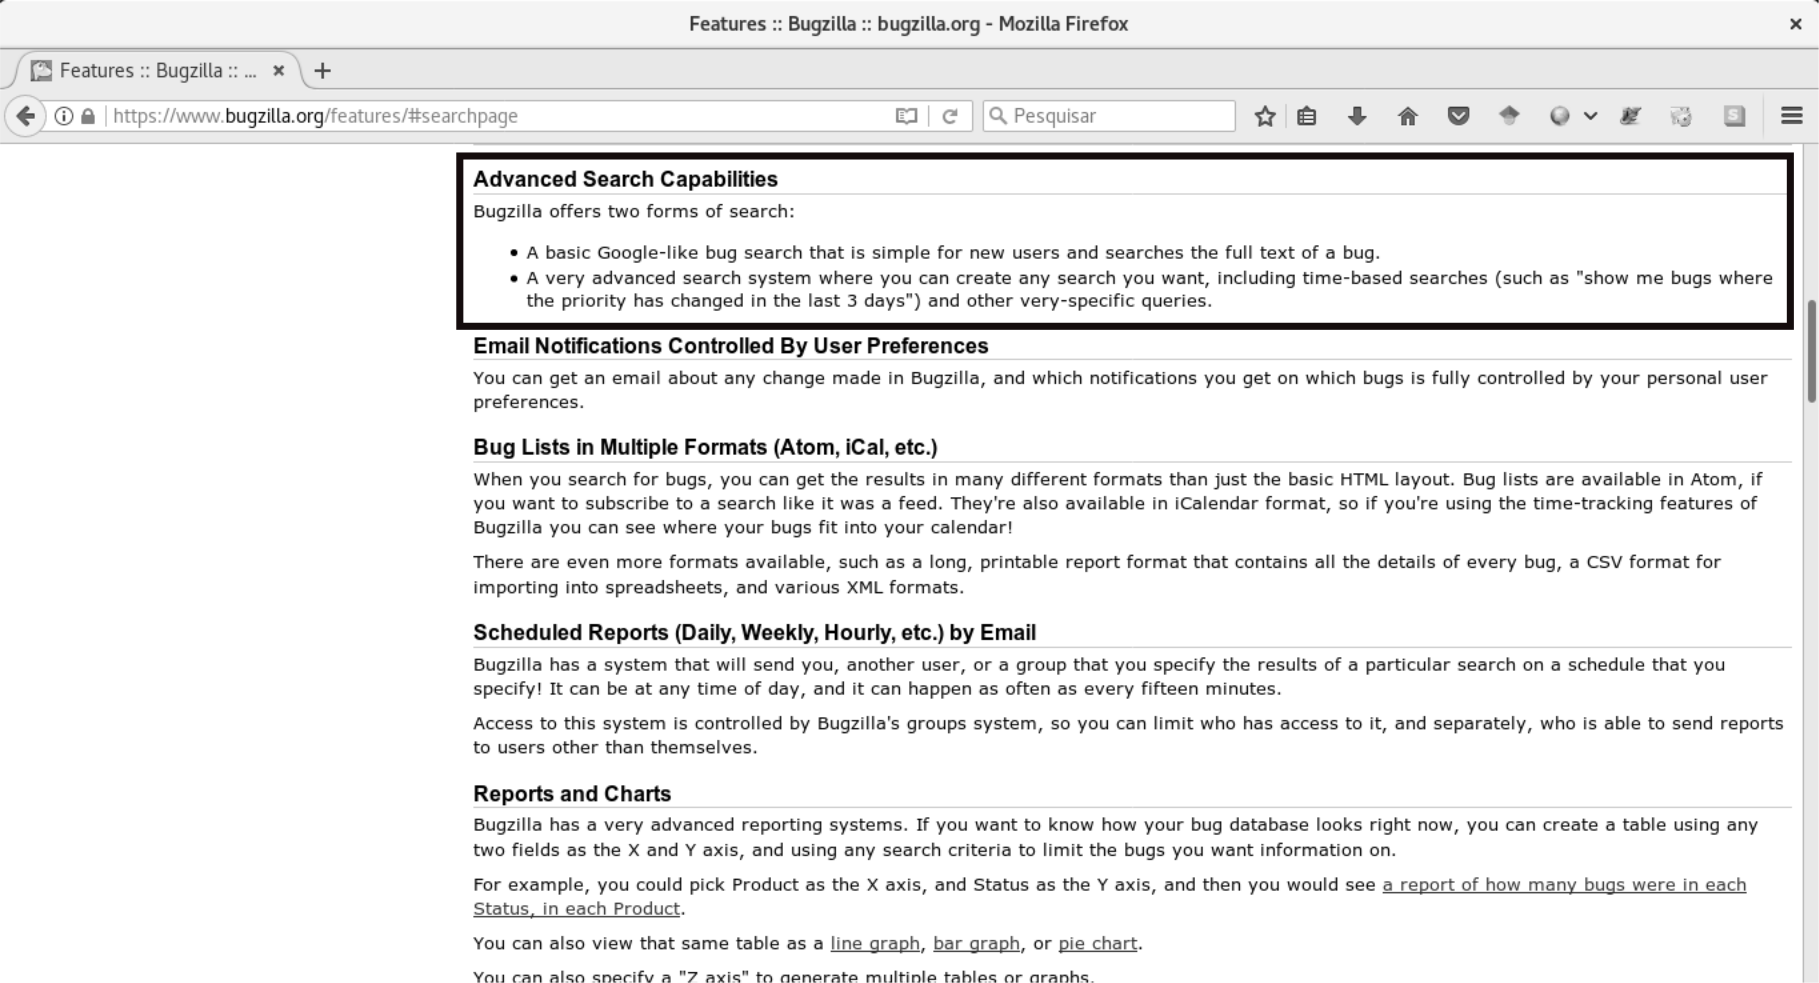
\includegraphics[width=1.0\linewidth]{./chapter-estudo-funcionalidades-fgrm/img/documentacao_bugzilla.png}
	\caption{Exemplo de documentação de uma funcionalidade do Bugzilla}\label{fig:documentacao_bugzilla}
\end{figure}

Os cartões foram organizados de modo a conter: o nome e a versão da ferramenta
analisada; a URL da documentação utilizada; o nome da funcionalidade coletada,
que consiste de uma descrição breve conforme existente na documentação;
descrição detalhada da funcionalidade, cujo objetivo é facilitar o processo de
agrupamento que será descrito na próxima seção. Nas
Figura~\ref{fig:documentacao_bugzilla} e~\ref{fig:exemplo_cartao_ordenado} é
possível visualizar, respectivamente, a documentação de uma funcionalidade da
ferramenta Bugzilla e o cartão produzido\footnote{O conteúdo integral dos
    cartões utilizados nesta dissertação estão disponíveis em
    \url{https://archive.org/download/dissertacao-vagner-clementino-um-estudo/cartoes-ordenados.csv}}

\begin{figure}[htpb]
	\centering
	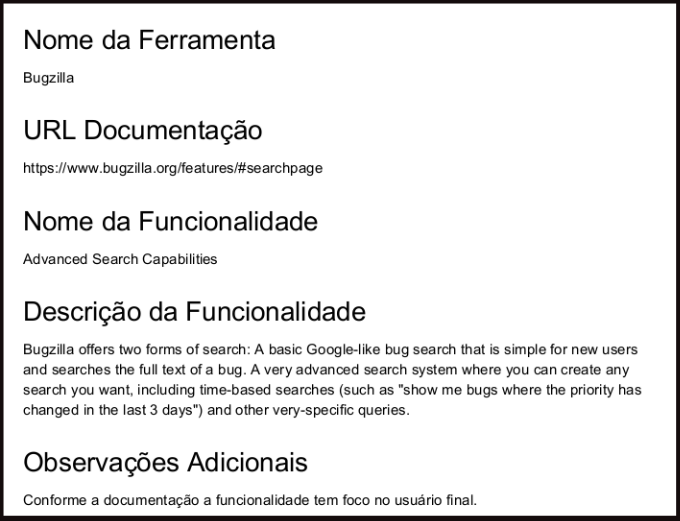
\includegraphics[width=0.9\linewidth]{./chapter-estudo-funcionalidades-fgrm/img/exemplo_cartao_ordenado.png}
	\caption{Exemplo de um cartão ordenado para uma funcionalidade da FGRM
		Bugzilla}\label{fig:exemplo_cartao_ordenado}
\end{figure}

\subsubsection{Agrupamento das Funcionalidades}\label{subsec:agrupamento_fucionalidades}

Esta etapa tem por objetivo agrupar as funcionalidades que aparecem com
nomenclatura distintas em diferentes ferramentas, mas que representam o mesmo
comportamento. Cabe ressaltar que o agrupamento de algumas funcionalidades pode
depender de uma análise interpretativa do responsável pela atividade. Neste
sentido, a fim de evitar algum tipo de viés, o agrupamento foi realizado em
duas etapas:

\begin{description}
	\item[Análise Individual] Nesta etapa o autor e um outro especialista
		realizam de forma separada os agrupamentos.
	\item[Anaĺise Compartilhada] Em um segundo momento tanto o autor quanto o
		es\-pe\-ci\-a\-lis\-ta discutem as possíveis divergências até que um
		consenso seja obtido.
\end{description}

Após o processo de agrupamento foi possível realizar a categorização das
funcionalidades das ferramentas. Os resultados do processo de agrupamento são
apresentados e discutidos nas próximas seções.

\subsection{Resultados}\label{sec:resultados}

Nesta seção iniciamos apresentando o perfil dos participantes do levantamento
que selecionou as ferramentas e em seguida exibimos as categorias resultantes do
processo de classificação dos cartões.

\subsubsection{Perfil dos Participantes}\label{ssub:perfil_participantes}

Ao final do levantamento obtivemos um total de \textit{52} respostas. Os
profissionais que participaram são em sua maioria desenvolvedores conforme pode
ser verificado na
Figura~\ref{fig:grafico_escolha_ferramentas_funcao_participantes}. O grupo de
respondentes também incluem Engenheiros de Software, Gerentes de Equipe e
Arquitetos de Software que, junto com os Desenvolvedores, representam mais de
80\% do total. Com relação à experiência verificamos que a maior parte possui
entre 3 e 10 anos (60\%). Na segunda posição temos os participantes com 10~-~20
anos de experiência (17\%). Quanto ao tamanho da equipe, verificamos uma
prevalência de equipes com mais de 10 membros, representando 38\% das
participações. As demais configurações de tamanho de equipe tiveram a seguinte
frequência de respostas: 2 a 5 membros (35\%); 6 a 10 membros (19\%); 1 membro
(8\%). Por sua vez, estas equipes estão predominantemente em empresas privadas
de software, é o caso de 37 participantes (74\%). Com relação ao local de
trabalho verificamos ainda que a segunda posição ficou para empresas que
pertencem ao setor governamental com 11 participantes (22\%). O restante é
composto por 01 profissional que se dedica a projetos de software livre (2\%) e
01 estudante (2\%).

\begin{figure}[htpb]
	\centering
	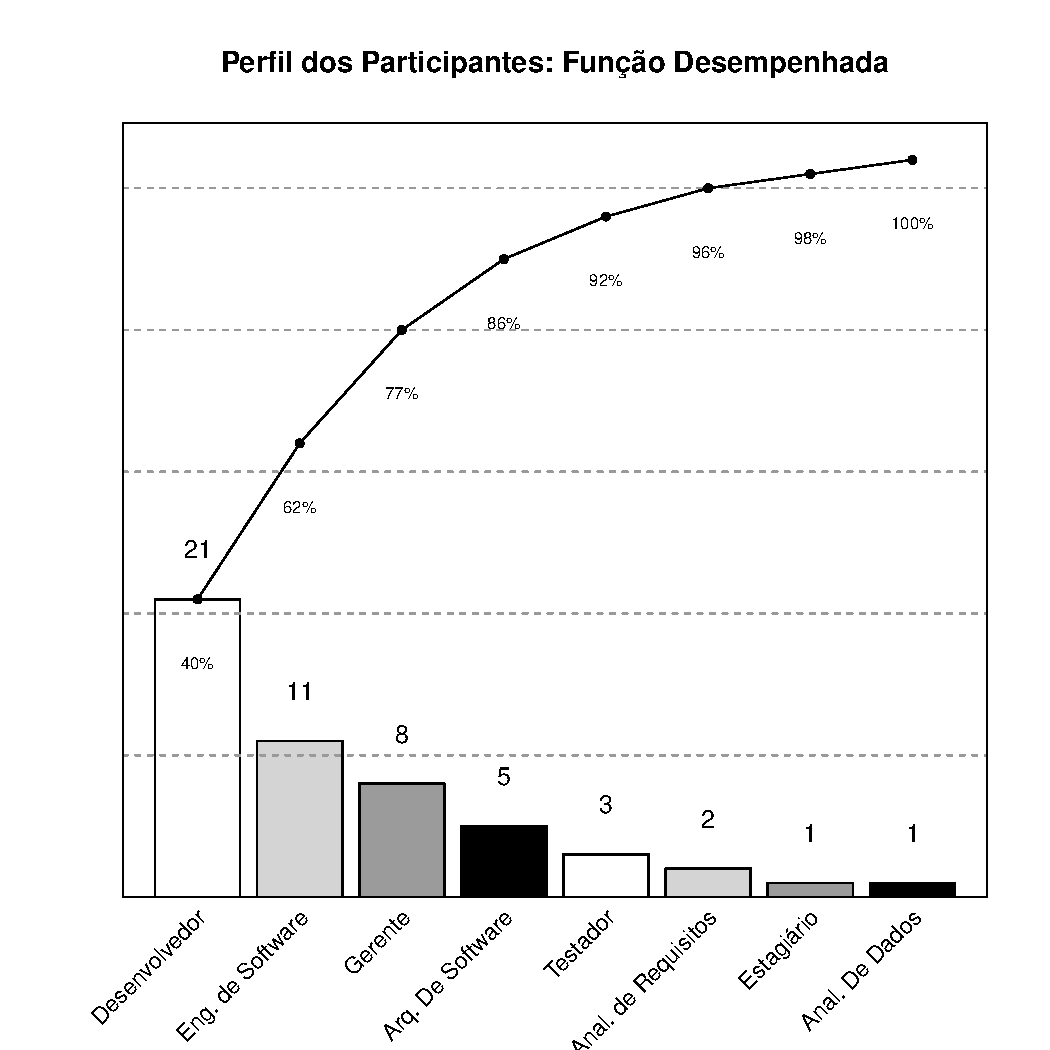
\includegraphics[width=0.7\linewidth]{./chapter-estudo-funcionalidades-fgrm/img/grafico_escolha_ferramentas_funcao_participantes.pdf}
	\caption{Funções desempenhadas pelos participantes}
\label{fig:grafico_escolha_ferramentas_funcao_participantes}
\end{figure}

\subsubsection{Ferramentas Escolhidas}
\label{subsec:resultados_ferramentas_escolhidas}

A partir do levantamento realizado e do processo de seleção descrito na
Seção~\ref{ssub:metodologia_criterios_selecao} obtivemos as ferramentas
apresentas na Tabela~\ref{tab:ferramenta_utilizadas_estudo}. Conforme pode ser
observado foram escolhidos três softwares que conforme os critérios que
adotamos podem ser classificados como ferramenta ou serviço da
Internet\footnote{A análise completa dos dados sobre a seleção das ferramentas
    pode ser encontrado em
    \url{https://archive.org/download/dissertacao-vagner-clementino-um-estudo/frequencia_selecao_ferramentas.csv}}.
É importante perceber que o \textit{Github} e o \textit{Gitlab} não estavam na
lista inicial, contudo, apareceram no resultado final. Isso decorre pelo fato
de optarmos por atribuir o peso 5 para ferramentas que foram citadas pelos
participantes de maneira espontânea.

\begin{table}[htpb]
\centering
\resizebox{\textwidth}{!}{%
\begin{tabular}{lccl}
\toprule
\multicolumn{1}{c}{\textbf{Ferramenta}} & \textbf{\textbf{Classificação}} &
\textbf{Versão} & \multicolumn{1}{c}{URL} \\
\bottomrule
Bugzilla & Ferramenta & 5.0.3 & https://www.bugzilla.org \\
Mantis Bug Tracker & Ferramenta & 1.3.2 & https://www.mantisbt.org \\
Redmine & Ferramenta & 3.3.1 & http://www.redmine.org/ \\
JIRA Software & Serviço & 7.2.4 & https://br.atlassian.com/software/jira \\
Github Issue System & Serviço & \@-\@ & https://github.com/ \\
Gitlab Issue Tracking System & Serviço & \@-\@ & https://gitlab.com/ \\ 
\bottomrule
\end{tabular}%
}
\caption{Ferramentas utilizadas no estudo}
\label{tab:ferramenta_utilizadas_estudo}
\end{table}

A Tabela~\ref{tab:fgrm-docs} apresenta as ferramentas e o elo de ligação para
os respectivos documentos que foram utilizados. Para aqueles sistemas que
apresentam documentação em mais de um i\-di\-o\-ma optamos por aquela escrita
em inglês por entendermos que poderia ser a mais atualizada.

\begin{table}[htpb]
\centering
\resizebox{\textwidth}{!}{%
\begin{tabular}{@{}ll@{}}
\toprule
\multicolumn{1}{c}{\textbf{Nome da Ferramenta}} & \multicolumn{1}{c}{\textbf{URL}} \\ \midrule
Bugzilla & \url{https://www.bugzilla.org/features/} \\
Github Issue Tracking System & \url{https://github.com/blog/411-github-issue-tracker} \\
Github Issue Tracking System & \url{https://github.com/features} \\
Github Issue Tracking System & \url{https://guides.github.com/features/issues/} \\
Gitlab Issue Tracking System & \url{http://docs.gitlab.com/ce/user/project/labels.html} \\
Gitlab Issue Tracking System & \url{https://about.gitlab.com/2016/08/22/announcing-the-gitlab-issue-board/} \\
Gitlab Issue Tracking System & \url{https://about.gitlab.com/solutions/issueboard/} \\
Gitlab Issue Tracking System & \url{https://docs.gitlab.com/ee/user/project/description\_templates.html} \\
Gitlab Issue Tracking System & \url{https://docs.gitlab.com/ee/user/project/issues/automatic\_issue\_closing.html} \\
Gitlab Issue Tracking System & \url{https://docs.gitlab.com/ee/workflow/issue\_weight.html} \\
Gitlab Issue Tracking System & \url{https://docs.gitlab.com/ee/workflow/milestones.html} \\
Gitlab Issue Tracking System & \url{https://docs.gitlab.com/ee/workflow/time\_tracking.html} \\
JIRA & \url{https://br.atlassian.com/software/jira/features} \\
MantisBT & \url{https://www.mantisbt.org/wiki/doku.php/mantisbt:features} \\
Redmine & \url{http://www.redmine.org/projects/redmine/wiki/Features} \\ \bottomrule
\end{tabular}%
}
\caption{Documentações utilizadas no processo de coleta de dados.}
\label{tab:fgrm-docs}
\end{table}

\subsubsection{Espectro de Funcionalidades das FGRMs}
\label{subsec:categorizacao_ferramentas}

Após a inspeção da documentação e validação dos dados obtivemos um total de 123
cartões, sendo eles sistematizados manualmente. Como o nosso objetivo é derivar
tópicos a partir de um conjunto inicial de cartões, optamos por realizar uma
\textit{classificação aberta}. Neste tipo de abordagem, os grupos são
estabelecidos durante o processo de classificação dos cartões em oposição a
outra forma de utilização da técnica em que a sistematização dos cartões ocorre
com base em grupos pré-determinados. Ao final do processo compilamos os tópicos
para construir um espectro de funcionalidades para as FGRMs exibido na
Figura~\ref{fig:diagrama-espectro-funcionalidades-fgrm}.

\begin{figure}[htpb]
	\centering
    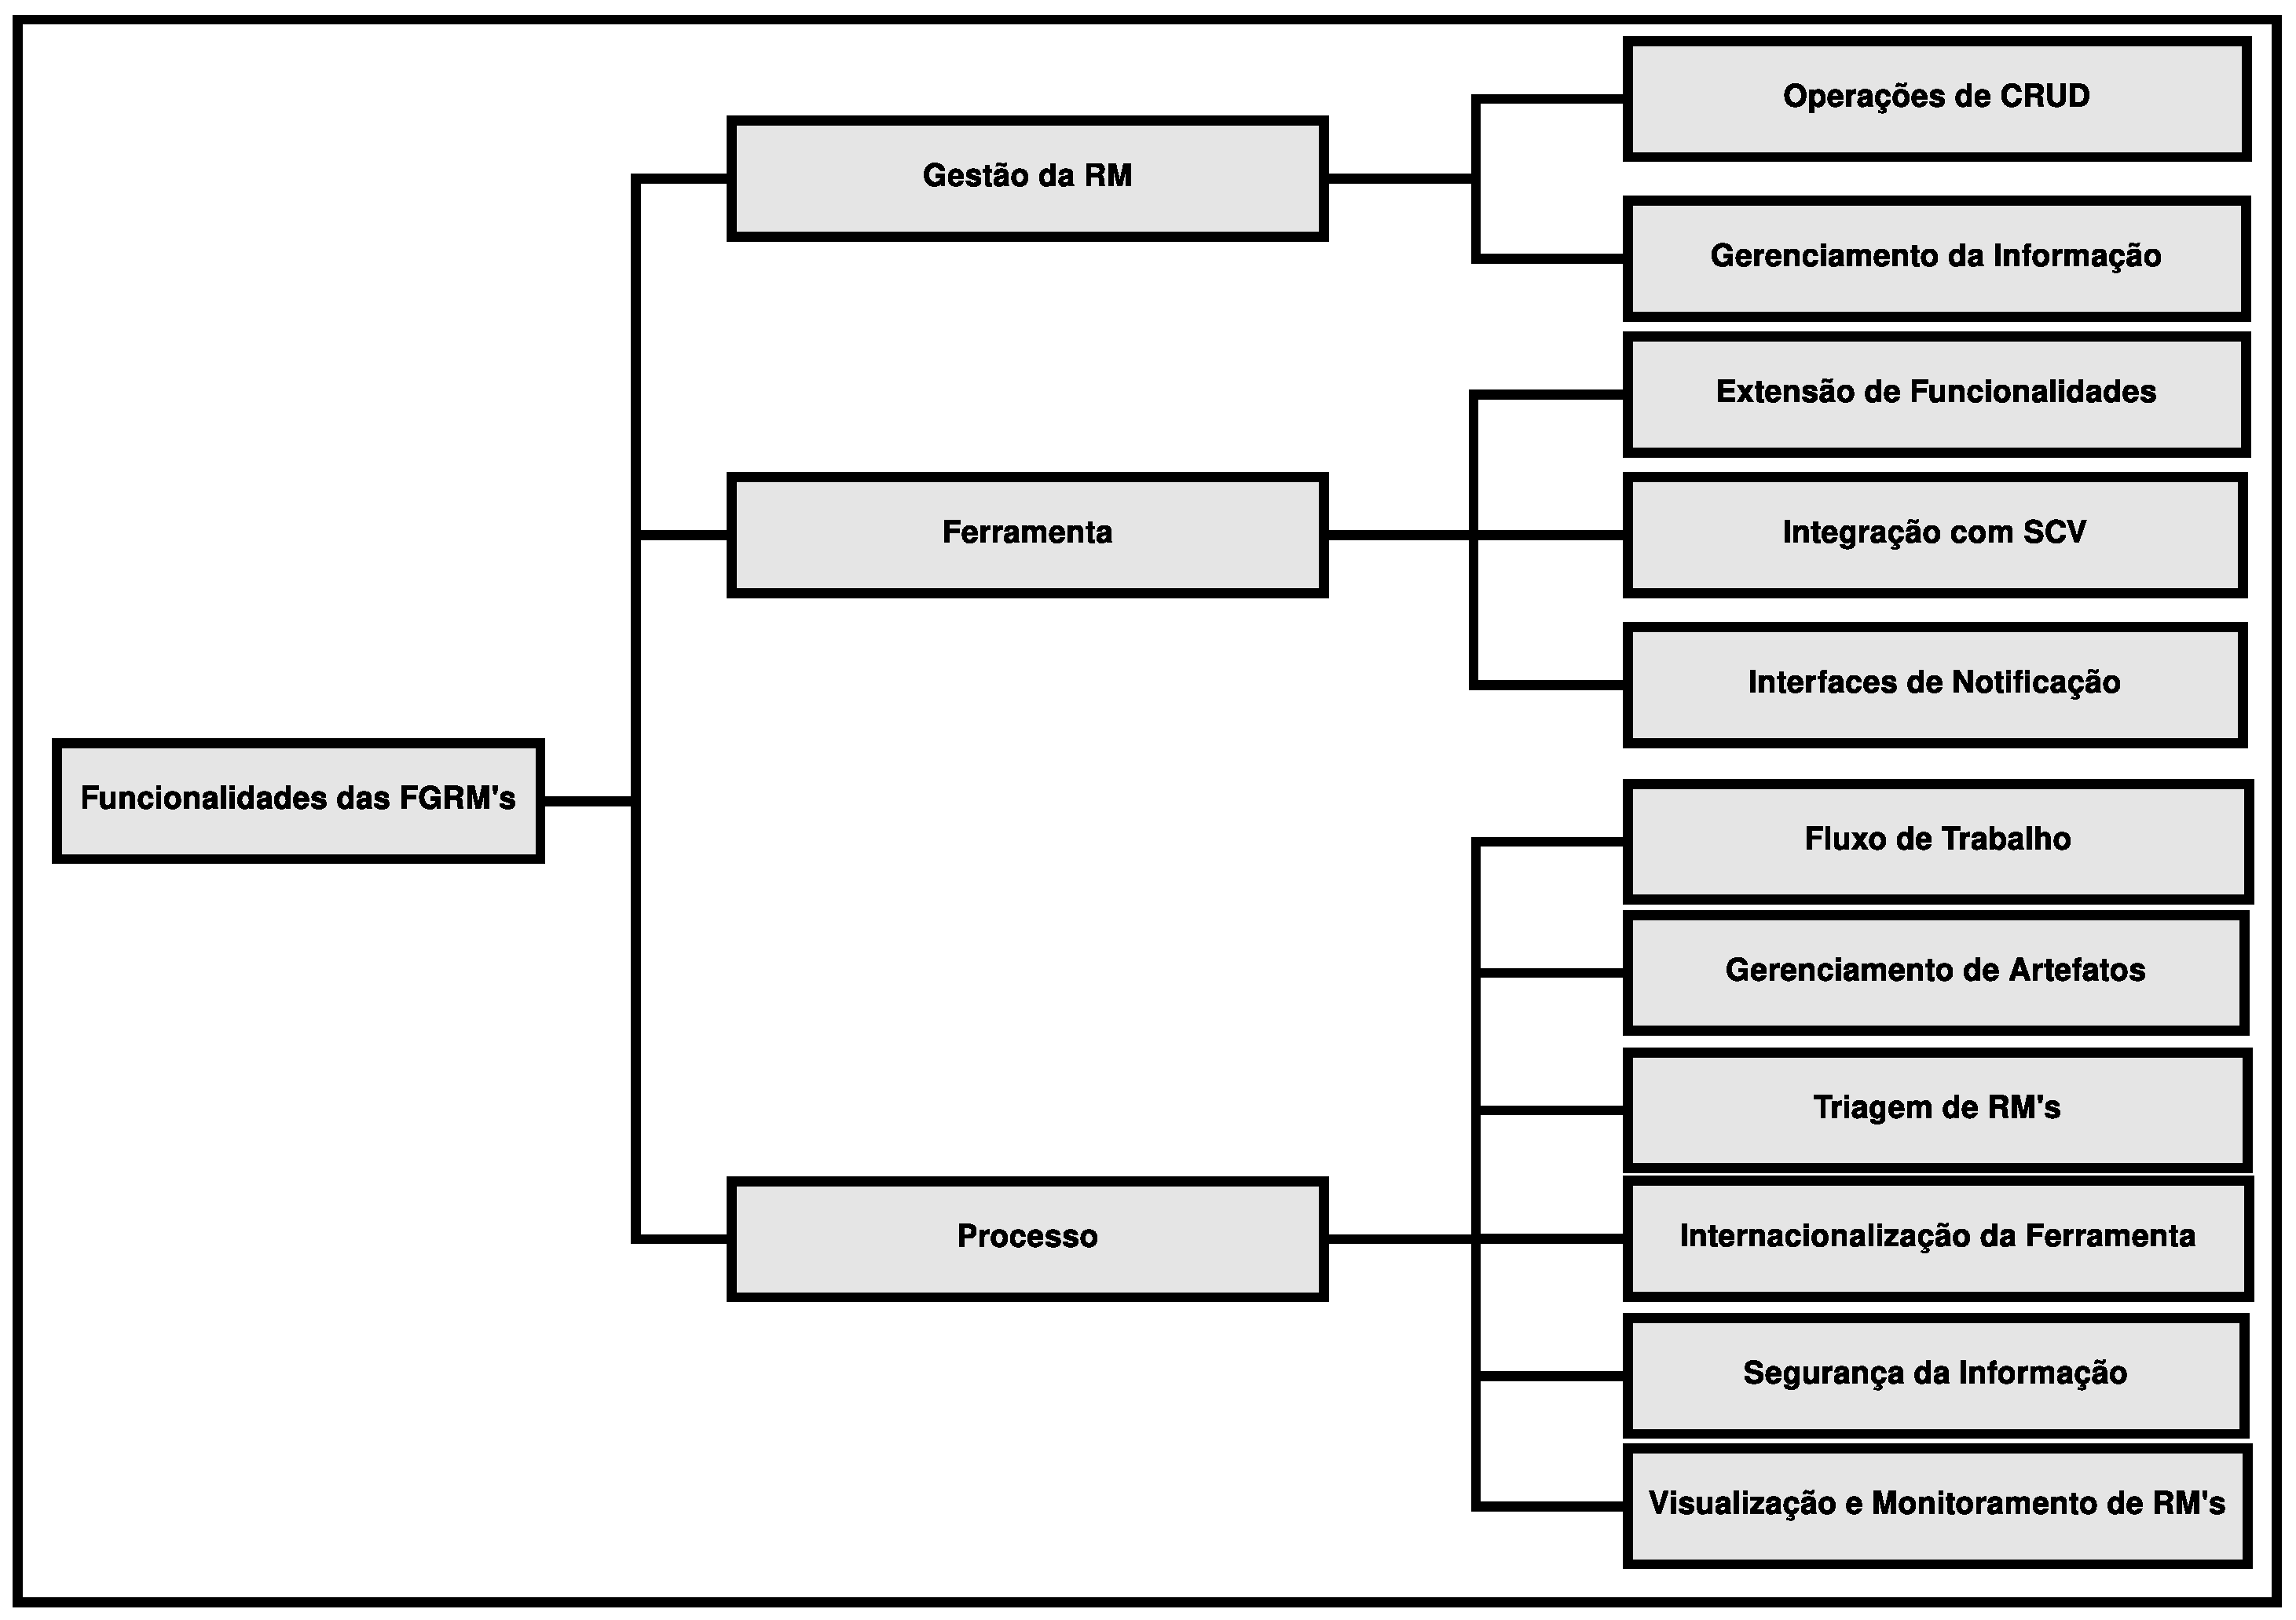
\includegraphics[width=1.15\linewidth]{./chapter-estudo-funcionalidades-fgrm/img/diagrama-espectro-funcionalidades-fgrm.eps}
	\caption{Modelo de funcionalidades básicas das FGRMs}
\label{fig:diagrama-espectro-funcionalidades-fgrm}
\end{figure}

A figura foi construída com base nas categorias de funcionalidades exibidas na
Tabela~\ref{tab:freq_categorias_cartoes} em que é possível verificar a
frequência que cada uma delas apareceu no conjunto de cartões coletados.

\begin{table}[htpb]
\centering
\resizebox{.7\textwidth}{!}{%
\begin{tabular}{lc}
\toprule
\multicolumn{1}{c}{\textbf{Categoria de Funcionalidades}} &
\textbf{\textbf{Frequência}} \\ 
\bottomrule
Operações de CRUD & 24 \\
Visualização e Monitoramento de RMs & 22 \\
Segurança da Informação & 17 \\
Fluxo de Trabalho & 15 \\
Interfaces de Notificação & 13 \\
Extensão de Funcionalidades & 8 \\
Triagem de RMs & 6 \\
Gerenciamento de Artefatos & 6 \\
Integração com Sistemas de Controle de Versão & 4 \\
Gerenciamento da Informação & 4 \\
Internacionalização da Ferramenta & 3 \\
Auditoria & 1 \\
\bottomrule
\end{tabular}%
}
\caption{Frequência de cada categoria de funcionalidade no conjunto de cartões
	obtidos.}
\label{tab:freq_categorias_cartoes}
\end{table}

A partir da Tabela~\ref{tab:freq_categorias_cartoes} é possível verificar que o
gerenciamento das RMs formam as funcionalidades mais frequentes das FGRMs\@. De
uma maneira geral, uma das primeiras responsabilidades de uma FGRM é gerir a
\textit{criação, consulta, atualização e destruição} de uma RM\@. Estas funções
podem ser agrupadas em um termo único denominado \textit{Operações de CRUD}
(acrônimo de \textit{Create}, \textit{Read}, \textit{Update} e \textit{Delete}
na língua Inglesa). Algumas das categorias apresentadas na
Tabela~\ref{tab:freq_categorias_cartoes} estão descritas descritas a seguir.

\paragraph{Operações de CRUD:}
\label{par:operações_de_crud}

Nesta categoria estão as funcionalidades que dão suporte à criação,	consulta,
atualização e destruição das RMs. Com relação à criação verificamos que algumas
FGRMs permitem a definição de \textit{campos personalizáveis} para o
preenchimento da RM\@. A ferramenta Bugzilla permite a criação de um campo
personalizado de modo a capturar informações específicas de um projeto. Estes
campos podem ainda ser exibidos com base no valor de outro, para usá-los apenas
quando for de interesse.

Esta categoria também agrupa as funcionalidades relacionadas à busca de RMs e à
localização de RMs duplicadas. Durante o processo de criação de uma RM, uma das
ferramentas possui a funcionalidade para detecção automatizada de duplicação de
RMs. Para criar RMs algumas ferramentas possibilitam diferentes
\textit{interfaces de entrada} de modo que ela possa ser criada através do
envio de e-mail, utilizando dispositivos móveis ou mediante formulários
disponíveis via Web\@.

Verificamos ainda que algumas FGRMs permitem que o relato da RM seja realizado
em linguagem com semântica de apresentação como o
Markdown\footnote{\url{https://en.wikipedia.org/wiki/Markdown}}, que permite,
dentre outras opções, a inclusão de código fonte com a sintaxe realçada. Isso
possibilita visualizar de forma mais clara partes do código que podem ser
incluídas no relato da RM\@. Neste mesmo tópico encontramos funcionalidades
para recuperação das RMs utilizando o texto contido no atributo que corresponde
ao relato, através de filtros personalizáveis ou por meio de uma Linguagem de
Domínio Específico (\textit{Domain-Specific Language} \@-\@ DSL) baseada em
SQL\@.

\paragraph{Gerenciamento da Informação:}
\label{par:gerenciamento_da_informação}

Dentro de um projeto de desenvolvimento ou manutenção de software gerenciar uma
RM por vez não é muito eficiente. Neste sentido, é necessário que as FGRMs
permitam o gerenciamento em massa da informação armazenada. Em geral, o
gerenciamento da informação fica a cargo dos Sistemas de Gerenciamento de Banco
da Dados \@-\@ \textit{SGBD}, neste sentido, a maior parte das funcionalidades
nesta categoria estão focadas em suportar múltiplos \textit{SGBDs}. Além disso,
a ferramenta Bugzilla oferece funcionalidade para validação de consistências
dos dados armazenados.

\paragraph{Extensão de Funcionalidades:}
\label{par:extensão_de_funcionalidades}

As FGRMs oferecem recursos que permitem que outras ferramentas possam interagir
e manipular a informação que elas armazenam. Nesta dimensão estão as
funcionalidades que possibilitam a manipulação externa dos dados contidos nas
RMs ou mesmo o desenvolvimento de novas funções ou comportamentos da FGRM
mediante o uso de interfaces de programação (APIs) e extensões.

As funcionalidades que compõem este grupo têm por objetivo estender o conjunto
de comportamentos oferecidos através de uma arquitetura de \textit{plug-in} ou
mediante o suporte de APIs. Algumas ferramentas como o Github permitem realizar
as atividades de gerência de uma RM mediante a utilização de uma API própria.
No caso do Bugzilla e do Mantis é permitido o acesso à informação das RMs
através de Webservices.

\paragraph{Integração com Sistemas de Controle de Versão:}
\label{par:integração_com_sistemas_de_controle_de_versão}

As FGRMs podem acessar os repositórios de código de fonte, gerenciados mediante
um Sistema de Controle de Versão (SCV), permitindo que o usuário navegue pelo
seu conteúdo, visualize e procure as alterações realizadas. As ferramentas
também possibilitam acesso aos diferentes tipos de SCV, tais como Git, SVN,
Mercurial.

\paragraph{Interfaces de Notificação:}
\label{par:interfaces_de_notificação}

Neste tópico estão as funcionalidades oferecidas pelas FGRMs para notificar as
diversas partes interessadas envolvidas em determinada RM\@. As FGRMs podem
notificar através de e-mail, RSS, Twitter e chats.

\paragraph{Fluxo de trabalho:}
\label{par:fluxo_de_trabalho}

Nesta categoria estão as funcionalidades que dão suporte às tarefas do
desenvolvimento e manutenção de software. Nela estão incluídos funções para
gerenciamento de tarefas e suporte a múltiplos projetos. Também é possível
personalizar o fluxo de trabalho adotado. Esta personalização é realizada
através da definição de \textit{situações} próprias que se adéquem às
necessidades do projeto de software.

\paragraph{Gerenciamento de Artefatos:}
\label{par:gerenciamento_de_artefatos}

O processo de trabalho relacionado com a manutenção de software pode consumir
ou gerar diversos artefatos, tais como documentos de requisitos, código fonte,
registros (logs) de teste e assim por diante~\cite{cavalcanti2013bug}. Em
alguns contextos, devido ao volume de artefatos gerados, é importante que a
FGRM forneça suporte para armazenamento e recuperação destes ativos
correspondentes ao processo de desenvolvimento de software. As FGRMs possuem
funcionalidades que se relacionam com a documentação de software,
geralmente no formato de Wikis. Além disso, algumas ferramentas permitem uma
melhor visualização de anexos da RM, como por exemplo arquivos no formato CSV
(comma-separated values).

\paragraph{Triagem de RMs:}\label{par:triagem_de_rm_s}

Este tópico descreve as funcionalidades relacionadas com a triagem de RMs. As
FGRMs dão suporte a esta atividade principalmente através da categorização das
RMs. Todas as ferramentas analisadas permitem algum tipo de classificação
através do uso de etiquetas previamente definidas.

\paragraph{Internacionalização da Ferramenta:}\label{par:internacionalização_da_ferramenta}

Neste tópico estão as características das FGRMs que ajudam no desenvolvimento
ou adaptação da interface para diferentes idiomas. As FGRMs possuem tradução
para diversos idiomas e também possuem funcionalidades que permitem aos
colaboradores criarem novas traduções.

\paragraph{Segurança da Informação:}
\label{par:segurança_da_informação}

Neste grupo estão as funcionalidades de uma FGRM que estão diretamente
relacionadas com proteção da informação no sentido de preservar o valor que
possui para um indivíduo ou uma organização. Assim as ferramentas oferecem
funcionalidades para suporte à confidencialidade, integridade e autenticidade
da informação armazenada.

\paragraph{Visualização e Monitoramento de RMs:}
\label{par:visualização_de_rm_s}

Em diversos contextos, devido ao volume das RMs, é importante que as partes
interessadas na manutenção do software, possam visualizar e monitorar a situação
das RMs que estão sendo analisadas. As FGRMs oferecem funcionalidades para
visualizar a informação das RMs mediante quadros similares àqueles utilizados
nas metodologias ágeis do tipo Kanban ou SCRUM\@. Existem funcionalidades que
permitem ao usuário visualizar um conjunto específico de RMs. Nesta mesma
categoria estão as funcionalidades para geração de relatórios para auxílio dos
tomadores de decisões.

\subsection{Discussão}
\label{sec:discussao}

Ao realizarmos a categorização dos cartões certos desafios se apresentaram. Para
algumas funcionalidades não há uma separação clara em qual categoria ela poderia
ser encaixada, como por exemplo a possibilidade que algumas FGRMs fornecem de
personalizar os campos que compõem uma RM\@. Esta função está relacionada com a
criação da RM (Operação de CRUD), contudo, também faz parte da definição do
processo de trabalho próprio de um projeto, o que permitiria categorizá-la como
Fluxo de Trabalho. Esta mesma situação ocorre com as funcionalidades de deleção
de uma RM que foram classificadas como \textit{Operações de CRUD}, mas que têm
relação com a categoria de \textit{Segurança da Informação} já que para realizar
tal ação o usuário deve ser identificado (login realizado no sistema) e estar
autorizado para realizar a ação.

A análise das funcionalidades nos permite verificar que o suporte oferecido
pelas FGRMs evoluíram da gerência simples de RMs para colaborar no processo de
desenvolvimento e manutenção do software. Entretanto, esta evolução não abrange
todo tipo de necessidade. As ferramentas analisadas apresentaram um suporte bem
estabelecido para atividades relativas à gestão da RM, como por exemplo a
criação de uma nova RM\@. Contudo, são bastante escassas as funções que
minimizem os problemas que ocorrem quando as RMs são criadas. Por exemplo não
foi possível verificar funcionalidades nativas das RMs que ajudem o responsável
pelo relato a fornecer as informações que serão necessárias à solução do que
está sendo pedido. Uma outra facilidade ausente neste tipo de ferramenta é a
identificação de possíveis RMs duplicadas.

Com base no resultado obtido foi possível verificar que as FGRMs oferecem
funcionalidades que dão suporte a todo o ciclo de vida de uma RM, conforme
discutido na Subseção~\ref{sub:fluxo_de_trabalho_requisicao_mudanca}. Todavia,
grande parte do esforço fica a cargo do usuário da ferramenta, o que pode
resultar em atrasos nas situações em que se têm muitas RMs para gerenciar. Um
exemplo deste problema ocorre no processo de atribuição do desenvolvedor
responsável por solucionar determinada RM\@ que é realizado de forma manual já
que as FGRMs não são capazes de ``recomendar'' o desenvolvedor mais apto.

Devido à sua importância, seria importante que as FGRMs incorporassem outros
comportamentos que ajudem no processo de desenvolvimento e manutenção de
software, especialmente em temas como busca de duplicados, melhoria da qualidade
do relato e atribuição e classificação automatizadas das RMs. As sugestões de
novas funcionalidades para as FGRMs são discutidas no
Capítulo~\ref{ch:sug_melhoria}.

\subsection{Ameaças à Validade}
\label{sec:ameacas_a_validade}

Em função da classificação ser uma atividade interpretativa, a classificação
das funcionalidades em si mesma é uma limitação desta dissertação. Uma outra
ameaça à validade do trabalho está no processo de seleção das ferramentas.
Apesar da escolha ter sido realizada com suporte de profissionais envolvidos em
manutenção de software, não podemos garantir que o número de respondentes nos
permite afirmar que escolhemos as ferramentas mais relevantes dentre aquelas
disponíveis. Além disso, a própria distribuição que compõe os participantes não
nos permite generalizar os resultados. Neste mesmo sentido, a fórmula que foi
utilizada para definir as mais relevantes podem conter um enviesamento
sobretudo pela forma que os pesos foram adotados, ou seja, não há como garantir
que o fato de um participante entender que uma determinada ferramenta é muito
relevante (peso igual a 5) mereça ser ponderado cinco vezes mais que uma outra
que não é conhecida (peso igual a 1).

Com relação à técnica de Cartões de Classificação temos dois pontos principais
de ameaças aos resultados. Como a extração dos dados foi realizada de forma
manual pode ter ocorrido algum tipo de equívoco no processo, como por exemplo a
não coleta de algum dado de determinada ferramenta por algum descuido. Todavia,
um número pequeno de ferramentas foi selecionado tendo em vista a limitação da
extração manual, o que pode ter minimizado este tipo de problema. Um segundo
ponto encontra-se na classificação dos cartões. Apesar do processo ter sido
realizado em pares pode ter ocorrido uma classificação de forma incorreta o que
pode acarretar em limitação dos resultados apresentados. Esta situação pode
ocorrer porque para algumas funcionalidades não há uma fronteira clara de qual
grupo ela poderia pertencer.

\section{Resumo do Capítulo}\label{sec:resumo_do_capitulo}

Neste capítulo discutimos o relacionamento da disciplina de Manutenção de
Software com as FGRMs. Para tanto apresentamos e discutimos os principais
conceitos relacionados e que são utilizados nos demais capítulos desta
dissertação. Além disso, apresentamos uma análise das funcionalidades das FGRMs
realizado com o suporte de um levantamento por questionário. A partir deste
levantamento foram obtidas as principais funções existentes nas FGRMs. O
conjunto comum de funcionalidades que foi encontrado é utilizado na dissertação
para discutir a proposição de novas funcionalidades ou melhorias das
existentes.
